\documentclass[a4paper, 11pt, french]{article}

\usepackage[french]{babel}
\usepackage[utf8]{inputenc}
\usepackage[T1]{fontenc}
\usepackage{csquotes}
\usepackage{amsmath,amsfonts,amssymb,mathrsfs}
\usepackage[includeheadfoot, hmargin=2cm, top=0.9cm, bottom = 1.8cm, headsep=2cm]{geometry}
\usepackage{lmodern} %pas pixelisé
\usepackage{engrec,titlesec,lipsum,xcolor}
\usepackage{fancybox}
\usepackage[skins, most]{tcolorbox}
\usepackage[bookmarks={true},bookmarksopen={true}, pdftitle={Cahier des charges}, pdfauthor={Chevalier Romain}, pdfsubject={Caméra domes}, colorlinks=true, linkcolor=black, urlcolor=blue, citecolor=black]{hyperref}
\usepackage{setspace}
\usepackage{stmaryrd}
\usepackage{multicol} 
\usepackage{enumitem}
\usepackage{array,multirow,makecell}
\usepackage{titlesec}
\usepackage{multirow}
\usepackage{hyperref}
\usepackage{listings}
\usepackage{graphicx}
\usepackage{caption}
\usepackage{subcaption}
\usepackage{float}
\usepackage{fancyhdr}
\usepackage[bottom]{footmisc}
\usepackage{footnote}
\usepackage[page,header]{appendix}
\usepackage{titletoc}
\makesavenoteenv{tabular}
\makesavenoteenv{table}

\graphicspath{{Figures/}{Photos/}}



\usepackage{tikz}
\usepackage{pgfplots}
\usetikzlibrary{decorations.pathmorphing, shapes, automata,positioning}

\usetikzlibrary{shapes.geometric, arrows}

\tikzstyle{process} = [rectangle, rounded corners, minimum width=2.5cm, minimum height=1cm, text centered, draw=black, fill=blue!10, font=\small]
\tikzstyle{decision} = [diamond, minimum width=2cm, minimum height=1cm, text centered, draw=black, fill=red!10]
\tikzstyle{sharedmem} = [rectangle, minimum width=2.5cm, minimum height=8cm, text centered, draw=black, fill=yellow!30]
\tikzstyle{startstop} = [rectangle, rounded corners, minimum width=3cm, minimum height=1cm,text centered, draw=black, fill=red!30]

\tikzstyle{arrow} = [thick,->,>=stealth]



%-----------------------------------------------------------------------------------

\pagestyle{fancy}
\renewcommand{\headrulewidth}{1pt}
\fancyhead[C]{\leftmark} 
%\fancyhead[R]{\includegraphics[scale=0.13]{logoAdeoService.jpg}}
\fancyhead[R]{
\includegraphics[scale=0.1]{Logo_CENTRALE_C.png}}
\newcolumntype{M}{>{\centering\arraybackslash}m{1.75cm}}
\setlength{\headheight}{30.5pt}

%-----------------------------------------------------------------------------------

\frenchbsetup{StandardLists=true}
%\setlength{\parskip}{1em}
\AddThinSpaceBeforeFootnotes
\FrenchFootnotes

%---------------------------------------------------------------
\lstset{
showstringspaces=false,
  aboveskip=2mm,
  belowskip=-5mm,
  backgroundcolor=\color{darkWhite},
  basicstyle=\ttfamily\small,
  breakatwhitespace=false,
  breaklines=true,
  captionpos=b,
  commentstyle=\color{vert},
  deletekeywords={...},
  escapeinside={\%*}{*)},
  framexleftmargin=10pt,
  framextopmargin=-1pt,
  framexbottommargin=0pt,
  %frame=tb,
  frame=trbl,
  emph={[8]\$, \texttildelow}, % nom des fonctions
  emphstyle={[8]\color{vert}},
  emph={[3]gcc, &}, % nom des fonctions
  emphstyle={[3]\color{blue}},
  keepspaces=true,
  keywordstyle=\color{blue},
  language=bash,
  literate=
  {²}{{\textsuperscript{2}}}1
  {⁴}{{\textsuperscript{4}}}1
  {⁶}{{\textsuperscript{6}}}1
  {⁸}{{\textsuperscript{8}}}1
  {€}{{\euro{}}}1
  {é}{{\'e}}1
  {è}{{\`{e}}}1
  {ê}{{\^{e}}}1
  {ë}{{\¨{e}}}1
  {É}{{\'{E}}}1
  {Ê}{{\^{E}}}1
  {û}{{\^{u}}}1
  {ù}{{\`{u}}}1
  {â}{{\^{a}}}1
  {à}{{\`{a}}}1
  {á}{{\'{a}}}1
  {ã}{{\~{a}}}1
  {Á}{{\'{A}}}1
  {Â}{{\^{A}}}1
  {Ã}{{\~{A}}}1
  {ç}{{\c{c}}}1
  {Ç}{{\c{C}}}1
  {õ}{{\~{o}}}1
  {ó}{{\'{o}}}1
  {ô}{{\^{o}}}1
  {Õ}{{\~{O}}}1
  {Ó}{{\'{O}}}1
  {Ô}{{\^{O}}}1
  {î}{{\^{i}}}1
  {Î}{{\^{I}}}1
  {í}{{\'{i}}}1
  {°}{{\textdegree}}1
  {Í}{{\~{Í}}}1,
  morekeywords={*,...},
  numbers=left,
  numbersep=3pt,
  numberstyle=\footnotesize\color{black},
  rulecolor=\color{black},
  showspaces=false,
  showstringspaces=false,
  showtabs=false,
  stepnumber=1,
  stringstyle=\color{orange},
  tabsize=4,
  title=\lstname,
}

% Configuration pour afficher du JSON
\lstdefinelanguage{json}{
    basicstyle=\ttfamily\small,
    numbers=left,
    numberstyle=\tiny\color{gray},
    framexleftmargin=10pt,
    framextopmargin=-1pt,
    framexbottommargin=0pt,
    belowskip=1mm,
    stepnumber=1,
    numbersep=2pt,
    showstringspaces=false,
    breaklines=true,
    frame=lines,
    backgroundcolor=\color{lightgray!20},
    literate=
     *{0}{{{\color{blue}0}}}{1}
      {1}{{{\color{blue}1}}}{1}
      {2}{{{\color{blue}2}}}{1}
      {3}{{{\color{blue}3}}}{1}
      {4}{{{\color{blue}4}}}{1}
      {5}{{{\color{blue}5}}}{1}
      {6}{{{\color{blue}6}}}{1}
      {7}{{{\color{blue}7}}}{1}
      {8}{{{\color{blue}8}}}{1}
      {9}{{{\color{blue}9}}}{1}
      {:}{{{\color{red}:}}}{1}
      {,}{{{\color{red},}}}{1}
      {\{}{{{\color{black}\{}}}{1}
      {\}}{{{\color{black}\}}}}{1}
      {[}{{{\color{black}[}}}{1}
      {]}{{{\color{black}]}}}{1},
}

%-----------------------------------------------------------------------------------

\definecolor{vert}{rgb}{0,0.69,0.31}
\definecolor{bleue}{rgb}{0,0.31,0.69} 
\definecolor{violet}{rgb}{0.38,0.18,055} % 97, 45, 140     244, 208, 63
\definecolor{jaune}{rgb}{0.96, 0.85, 0.23}

\definecolor{darkWhite}{rgb}{0.94,0.94,0.94}
\definecolor{vert}{rgb}{0,0.69,0.31}
\definecolor{rose}{rgb}{1,0.08,0.58}% rgb(255,20,147)
\definecolor{rouge}{rgb}{0.78,0.12,0.08}
\definecolor{gris}{rgb}{0.4,0.4,0.4}
\definecolor{marron}{rgb}{0.4,0.2,0}
\definecolor{darkWhite}{rgb}{0.94,0.94,0.94}

%-----------------------------------------------------------------------------------

\title{%
        \Huge Suivi d'un grimpeur par caméra dome \\
        \LARGE Rapport de PDI}

\author{\LARGE CHEVALIER Romain}
\date{\today}

\newcommand{\hsp}{\hspace{20pt}}
\newcommand{\HRule}{\rule{\linewidth}{0.5mm}}

%-----------------------------------------------------------------------------------

\newcounter{obj}
\setcounter{obj}{1}

%-----------------------------------------------------------------------------------

\usepackage[backend=biber,style=numeric,sorting=none]{biblatex}
\addbibresource{bibliographie.bib} % Fichier contenant les références


%-----------------------------------------------------------------------------------

\pgfplotsset{compat=1.18}


\begin{document}
\pagenumbering{roman}
\begin{titlepage}

    \begin{titlepage}
        \begin{center}
      
          % Upper part of the page. The '~' is needed because \\
          % only works if a paragraph has started.
      
          \textsc{\LARGE École Centrale De Lille}\\[2cm]
      
          \textsc{\huge Projet d'intégration}\\[2cm]
      
          % Title
          \HRule \\[0.4cm]
          { \Huge \bfseries Suivi d'un grimpeur par caméra dome\\[0.4cm] }
      
          \HRule \\[2cm]

          \textsc{\Large Rapport de PDI \\} {\large\today}\\[1.5cm]
          
          \vfill
          % A cahnger pour les caméras installées 
          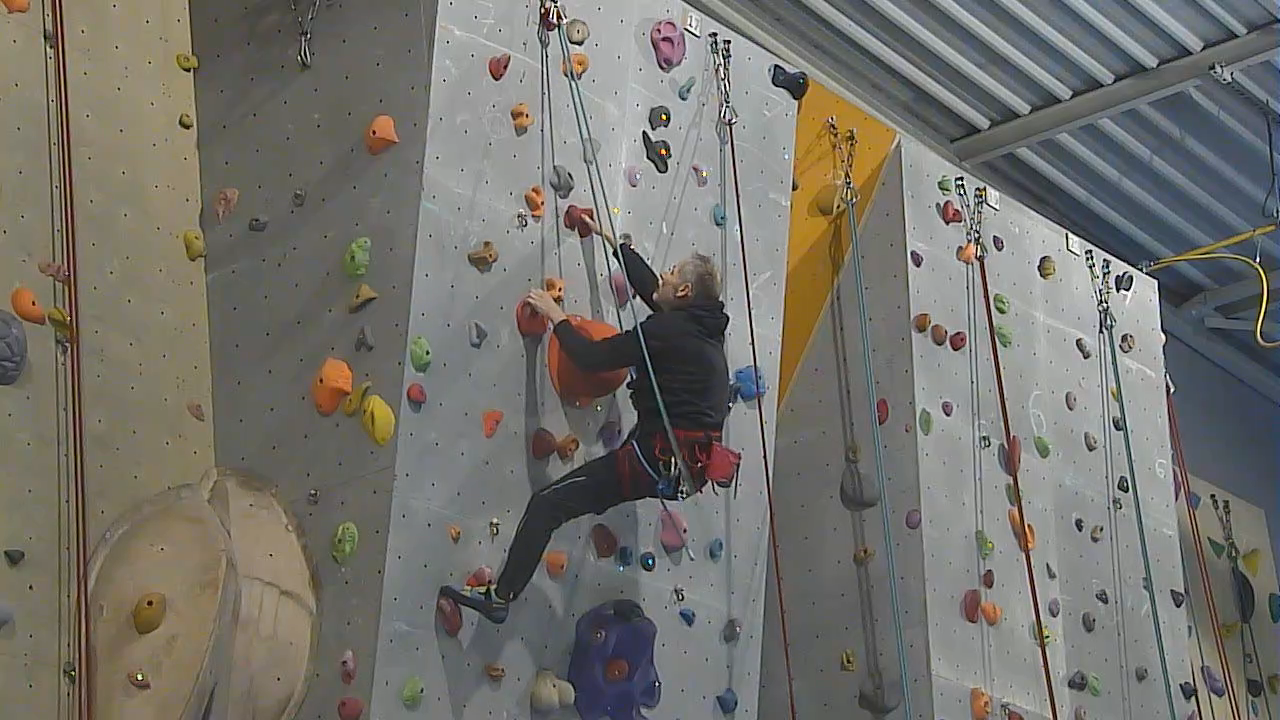
\includegraphics[width=.8\textwidth]{exemplePaysage.png}
          \vfill
 
          % Author and supervisor
          \begin{minipage}{0.4\textwidth}
            \begin{flushleft} \large
              CHEVALIER Romain\\
            \end{flushleft}
          \end{minipage}
          \begin{minipage}{0.4\textwidth}
            \begin{flushright} \large
              \emph{Tuteur :}  BOURDEAUD'HUY T. \\
            \end{flushright}
          \end{minipage}
      
          \vspace{1cm}
         
        \end{center}
      \end{titlepage}
    
    \normalsize
   
\end{titlepage}

%-----------------------------------------------------------------------------------

\setcounter{secnumdepth}{3}
\setcounter{tocdepth}{3}
\startcontents[sections]

%-----------------------------------------------------------------------------------
\tableofcontents
%\printcontents[sections]{l}{1}{\setcounter{tocdepth}{3}}
%\printcontents[sub]{l}{1}{\setcounter{tocdepth}{2}}
\pagenumbering{arabic}
\newpage

%-------------------------------------------------------------

\section{Contexte}
Afin d'améliorer les services offerts aux utilisateurs de la salle d’escalade \textit{Sac à Pof} situé à  Mons-en-Barœul (59), on envisage de mettre en place un système de suivi automatisé des grimpeurs à l'aide de caméras IP dômes motorisées. Ces caméras permettront de suivre les mouvements des grimpeurs sur les différentes voies en ajustant automatiquement le cadrage et le zoom en fonction de leur position. Le service sera accessible via une application web hébergée sur un serveur local. Cette solution vise à offrir un support d'analyse post-session, afin de permettre aux grimpeur de comprendre leurs forces et faiblesses pour s'améliorer.

Afin de réaliser ce projet, nous sommes en possession de deux caméras IP dômes motorisées de la marque \textit{AXIS} modèle \textit{Q6304-E\footnote{Voir \href{https://www.axis.com/dam/public/11/e4/20/cam\%C3\%A9ra-r\%C3\%A9seau-\%C3\%A0-d\%C3\%B4me-ptz-axis-q6034-e-fr-FR-201515.pdf}{fiche technique} pour plus d'informations}}, d'un routeur, d'une tablette Android et d'un reTerminal qui contient un raspberry pi 4, un écran HD de 5 pouces et une mémoire interne de 32 Go \cite{reTerminal}.

\subsection{Objectifs}
Les objectifs de ce projet sont multiples et  résumés dans la liste suivante :
\begin{itemize}
  \item Prendre en main les caméras IP dômes motorisées et les intégrer dans un réseau local.
  \item Développer une interface web permettant de piloter les caméras, l'enregistrement de  \item Avoir un retour visuel de la caméra en temps réel sur l'interface web.
  \item Développer une méthode de communication entre l'application web et les programmes de contrôle des caméras.
  \item Développer un algorithme de suivi de grimpeur en temps réel.
  \item Développer une méthode permettant d'enregister sur un stockage une vidéo.
  \item Avoir une application modulable permettant de modifier les caméra et les paramètres de détection.
\end{itemize}

\section{Architecture du système}
\subsection{Architecture matérielle}
Le système est composé de plusieurs éléments qui interagissent entre eux, la figure \ref{fig:architecture} montre l'architecture du système. Le système repose sur un \textbf{Raspberry Pi 4}, qui joue un rôle central en assurant la communication entre les différentes composantes. Il est connecté au réseau local via un \textbf{routeur}, qui agit comme un serveur DHCP, attribuant dynamiquement les adresses IP aux appareils du système.

Les \textbf{caméras Dome IP} sont accessibles via HTTP et envoient leur flux vidéo vers le Raspberry Pi lorsqu’elles sont activées. Ces caméras disposent de positions prédéfinies correspondant aux différentes voies d’escalade, mais peuvent également être orientées dynamiquement par l’utilisateur via la \textbf{tablette} fournie ou tout autre appareil connecté au réseau local.

Le Raspberry Pi exécute un serveur d’application web,ce serveur permet :
\begin{itemize}
    \item de piloter les caméras (changement de position, orientation manuelle),
    \item de gérer les enregistrements vidéo,
    \item de stocker dans une base de données les vidéos enregistrées ainsi que les positions des caméras définies par l’utilisateur.
\end{itemize}

L’enregistrement des vidéos est déclenché manuellement depuis l’interface de la tablette et les fichiers sont conservés jusqu’à suppression par l’utilisateur.

L’architecture ainsi mise en place assure une gestion centralisée et accessible du système, tout en permettant un contrôle précis et flexible des caméras et des enregistrements.


\begin{figure}[!ht]
  \centering
  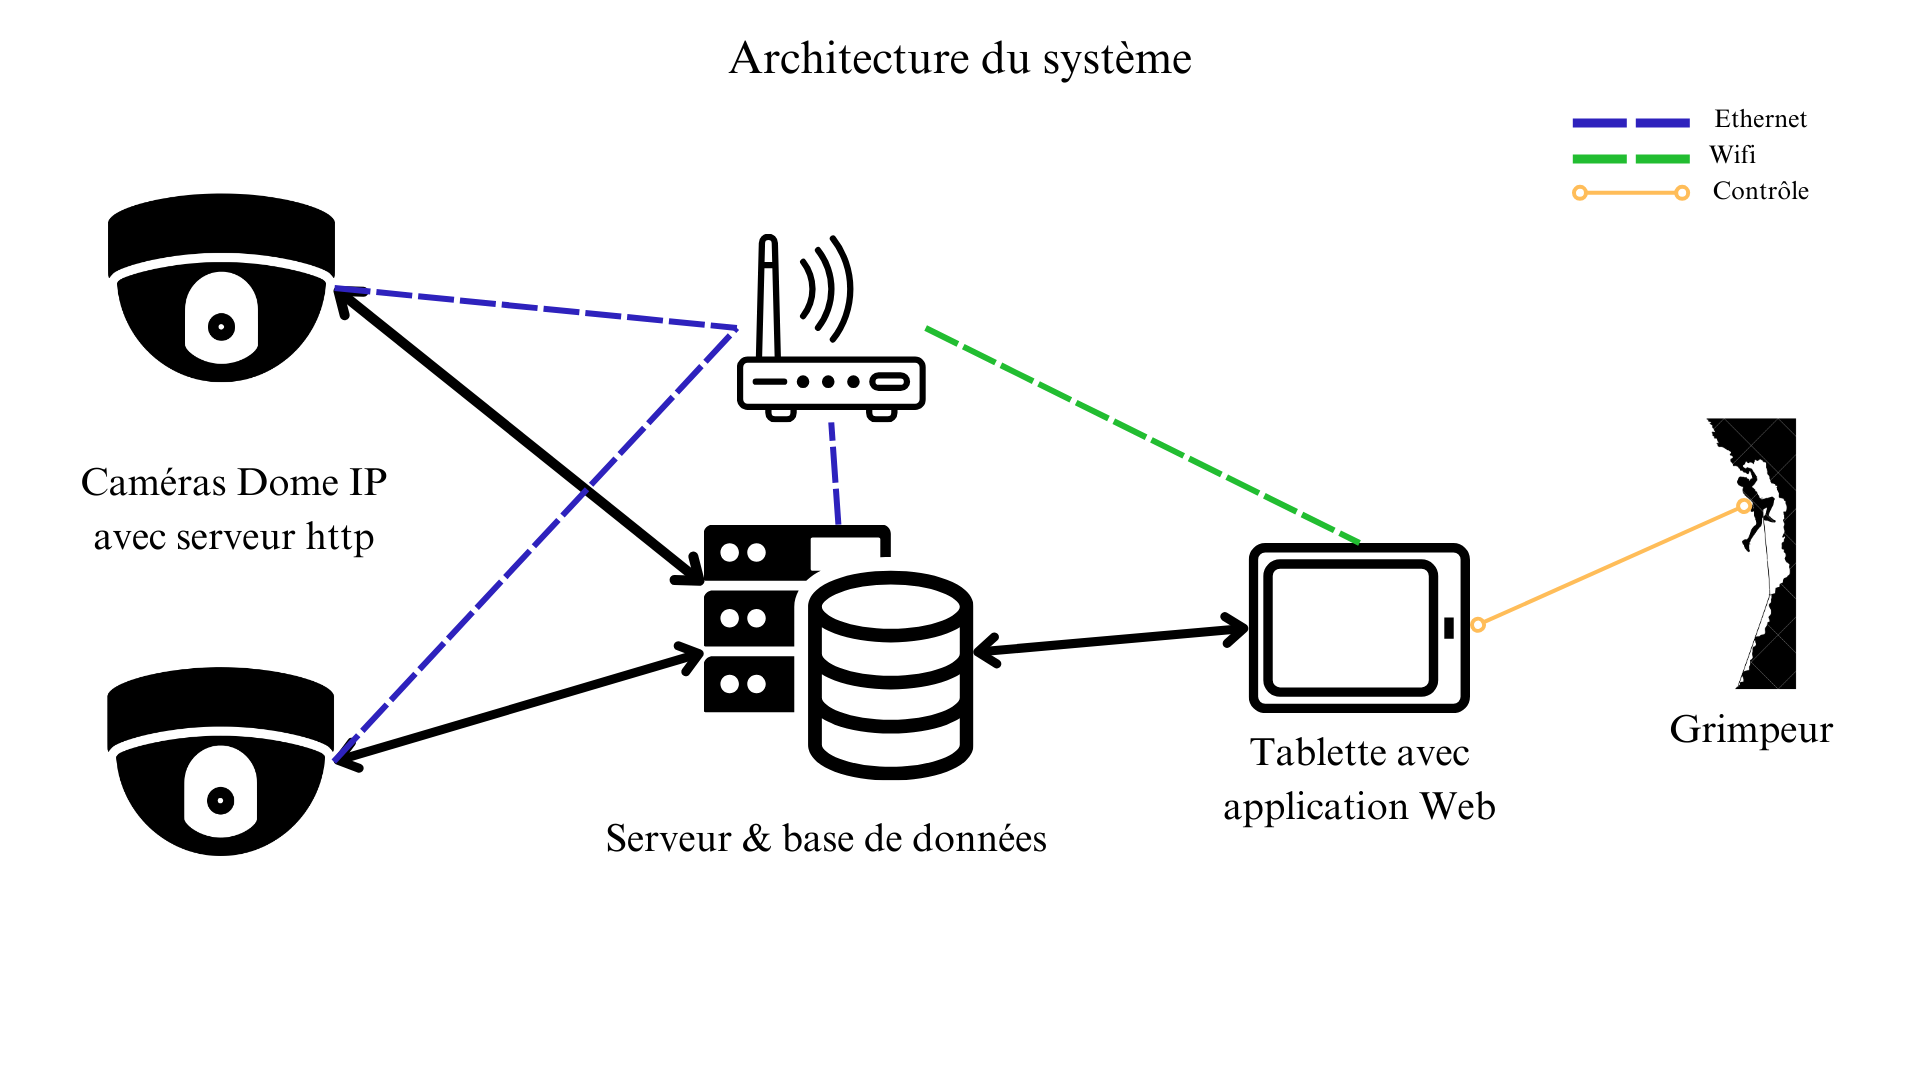
\includegraphics[width=\textwidth]{architectureMaterielle.png}
  \caption{Architecture du système}
  \label{fig:architecture}
\end{figure}

\subsection{Architecture logicielle}
L'architecture logicielle du système est représentée sur la figure \ref{fig:architectureLogicielle}. Le raspberry Pi divise ses tâches en deux parties distinctes : le serveur web et la partie gestion de l'application développée. En fonction des actions effectuées sur la page web, le serveur apache exécuté deux programmes \texttt{CGI} (Common Gateway Interface) différents, le premier programme, nommé \textbf{video.cgi} codé en \texttt{c++}, démarre au chargement de la page permet d'afficher le flux vidéo de la caméra sur la page web en lisant les images brutes dans la mémoire partagée et en les encodant en \texttt{JPEG}. Le second (\textbf{action.cgi} développé en \texttt{c}) permet de transmettre les ordres de déplacement de la caméra ou lancer un enregistrement vidéo via l'écriture de cet ordre dans un segment de mémoire partagé puis de réveillé le programme principal en lui envoyant un signal. 


De l'autre côté, le programme principal (\textbf{main} programmé en \texttt{c}) est en charge de la gestion des caméras, de la détection de mouvement et de l'enregistrement des vidéos. Au démarrage, il crée un processus fils (\textbf{écriture mémoire})qui est en charge de récupérer le flux vidéo du serveur HTTP de la caméra et de le stocker en image brute dans une mémoire partagée. Le programme principal est ensuite en attente d'un signal pour effectuer une action, comme le déplacement de la caméra, l'enregistrement de position ou encore le lancement d'un enregistrement qui va crée un processus fils (\textbf{enregistrement vidéo}) qui encode le flux video en \texttt{MP4} afin de le stocker sur le disque dur et lance la détection du grimpeur pour suivre ces mouvements à l'aide d'un second fils (\textbf{détection}). Ces deux processus récupèrent les images en lisant la mémoire partagée et les traitent pour effectuer leur tâche. Enfin, le programme de détection peut directement agir sur la position de la caméra en lui envoyant une requête HTTP.


\begin{figure}[!ht]
  \centering
  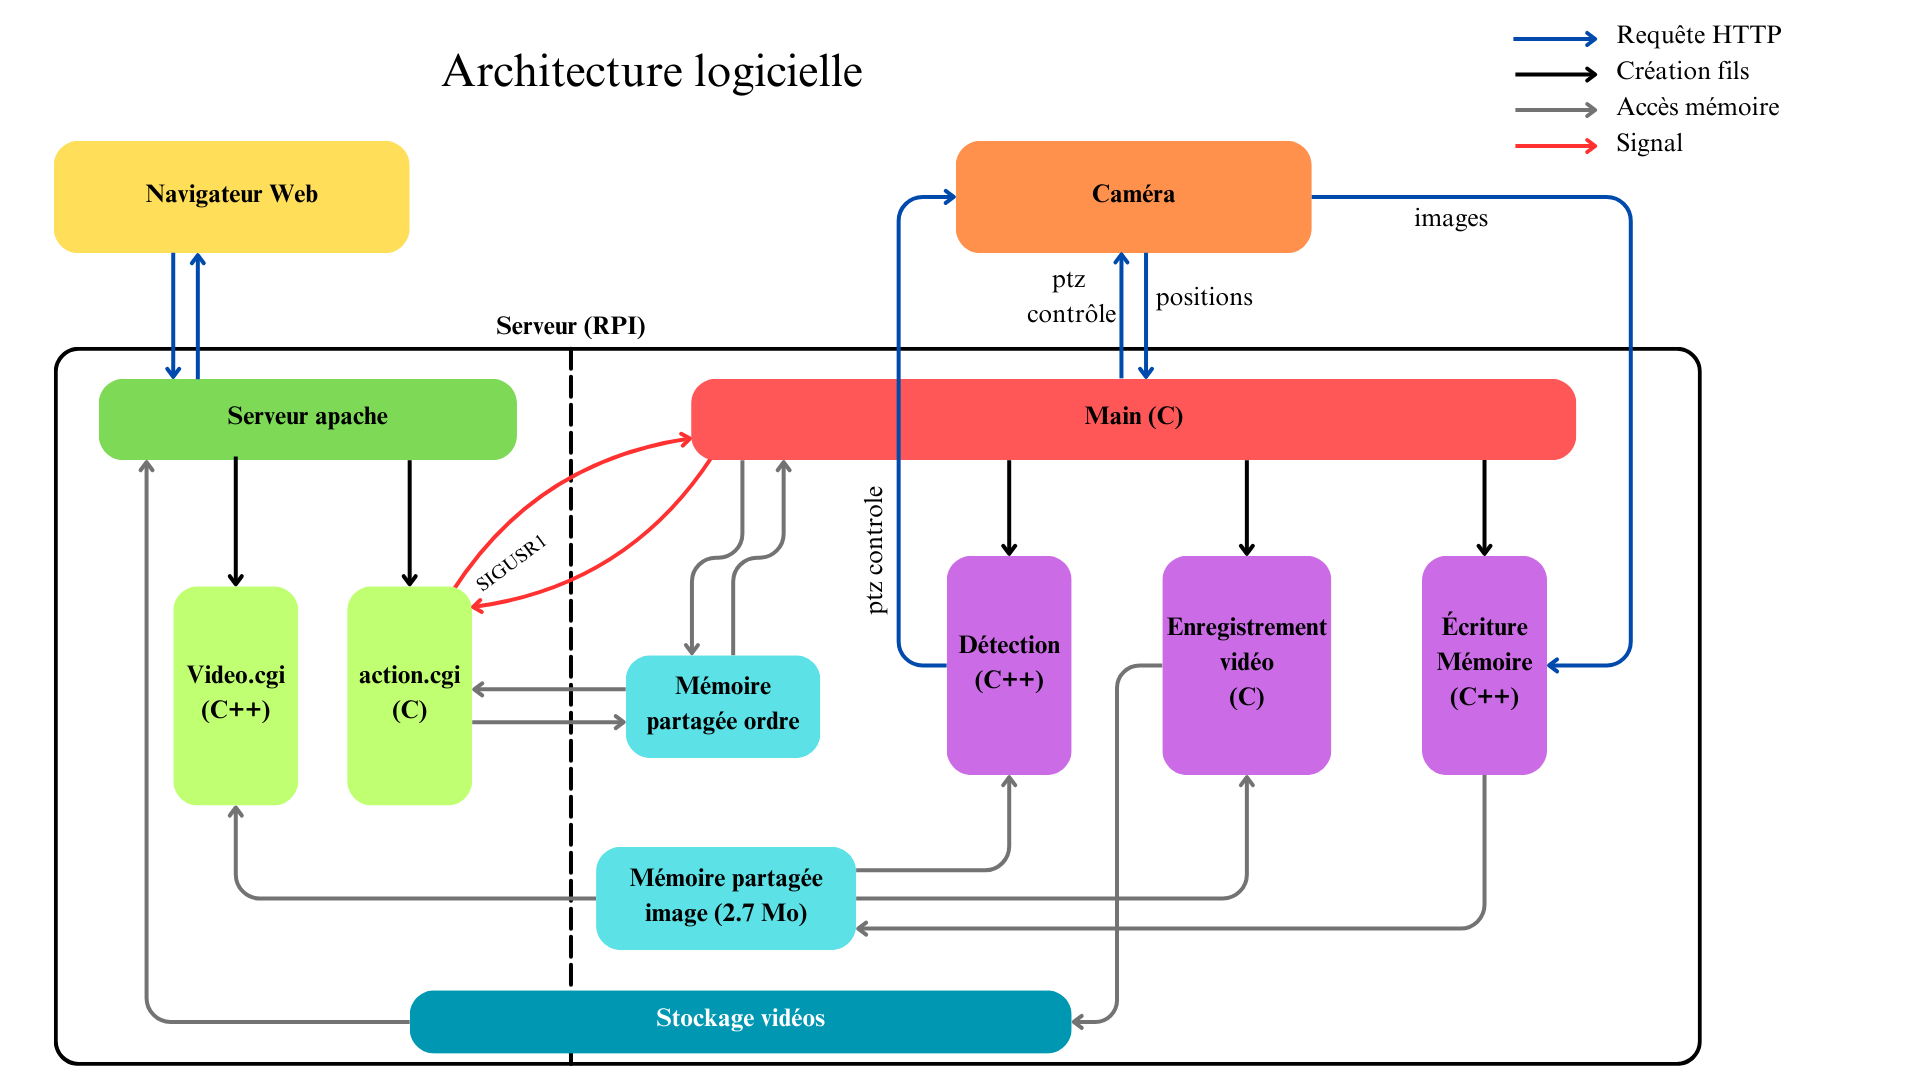
\includegraphics[width=\textwidth]{architectureLogicielle.png}
  \caption{Architecture logicielle}
  \label{fig:architectureLogicielle}
\end{figure}


%-----------------------------------------------------------

\section{Développement de l'application}
Dans cette partie, nous allons détailler les différentes étapes de développement de l'application pour chaque brique du système présent dans l'architecture logicielle en figure \ref{fig:architectureLogicielle}. Tout le code source est disponible sur le dépôt \href{https://github.com/Romaiiin91/suiviGrimpeur_PDI}{GitHub}.

%-----------------------------------------------------------
\subsection{Application système}

La partie système de l'application est composée de plusieurs fichiers et programmes qui interagissent pour gérer les caméras, les enregistrements vidéo et la communication avec l'interface web. 

\subsubsection{Programme principal}

Le fichier \texttt{main.c} constitue le cœur du système de gestion des caméras et de la communication inter-processus. Il est responsable de l'initialisation des caméras, de la gestion des enregistrements vidéo, de la détection des mouvements, et de l'interaction avec l'interface CGI via des segments de mémoire partagée et des sémaphores.

\paragraph{Initialisation du programme}
Lors de son démarrage, le programme effectue plusieurs étapes d'initialisation :
\begin{itemize}
    \item \textbf{Gestionnaire de fin d'exécution} : La fonction \texttt{atexit(bye)} garantit que toutes les ressources (mémoire partagée, sémaphores, processus enfants) sont correctement libérées à la fin du programme.
    \item \textbf{Initialisation des sémaphores} : La fonction \texttt{initSemaphores()} crée des sémaphores nommés pour synchroniser les processus et gérer l'accès à la mémoire partagée, voir le paragraphe~\ref{par:semaphores} pour leur fonctionnement.
    \item \textbf{Initialisation de la mémoire partagée} : La fonction \texttt{initSegmentMemoire()} configure deux segments de mémoire partagée : un pour les ordres envoyés par l'interface CGI et un autre pour stocker les images brutes capturées par les caméras.
    \item \textbf{Initialisation des caméras} : La fonction \texttt{initCamera()} charge les paramètres des caméras depuis un fichier JSON et configure les caméras actives. Ce fichier contient le numéro de la caméra, son adresse IP et son orientation, voir listing~\ref{lst:camerasSettings} pour un exemple de fichier de configuration.
    Afin que le système puisse s'adapter à l'orientation de la caméra (portrait, paysage, portrait renversé ou paysage renversé), la fonction \texttt{setParamCamera} vient définir les paramètre de la caméra pour que le système puisse s'adapter automatiquement. En effet, on definit le mouvement d'inclinaison et le mouvement panoramique en fonction de l'orientation (par exemple, pour le mode paysage un déplacement vers le haut correspond à une augmentation de l'angle d'inclinaison et le mode portrait renverse correspond a une diminution de l'angle panoramique). Un exemple de fichier de configuration est donné dans le listing~\ref{lst:cameraActive} pour la caméra 1 en paysage.
\end{itemize}

\begin{lstlisting}[language=json, caption={Fichier json pour définir les caméras, \texttt{cameras.json}}, label={lst:camerasSettings}]
{
    "1": {
        "IP": "192.168.10.21",
        "orientation": 90
    },
    "2": {
        "IP": "192.168.10.22",
        "orientation": 270
    }
}
\end{lstlisting}

\begin{lstlisting}[language=json, caption={Fichier json pour partager la caméra active, \texttt{cameraActive.json}}, label={lst:cameraActive}]
{
    "id": 1, 
    "IP": "192.168.1.13", 
    "orientation": 0, 
    "height": 720, 
    "width": 1280, 
    "up": 1, 
    "down": -1, 
    "left": -1, 
    "right": 1, 
    "cmdVertical": "rtilt", 
    "cmdHorizontal": "rpan"
}
\end{lstlisting}

\paragraph{Gestion des signaux}
Le programme installe un gestionnaire de signaux (\texttt{signalHandler}) pour répondre aux événements suivants :
\begin{itemize}
    \item \textbf{SIGINT} : Interruption manuelle (Ctrl+C) pour arrêter le programme proprement.
    \item \textbf{SIGCHLD} : Gestion des processus enfants terminés pour éviter les processus zombies.
    \item \textbf{SIGUSR1} : Signal utilisé pour indiquer qu'un nouvel ordre a été reçu via la mémoire partagée.
\end{itemize}

\paragraph{Boucle principale}
Le programme entre dans une boucle infinie en appelant \texttt{pause()}, ce qui le met en attente d'un signal. Lorsqu'un signal est reçu, le gestionnaire de signaux (\texttt{signalHandler}) est exécuté pour traiter l'événement.

\paragraph{Gestion des ordres}
Lorsqu'un signal \texttt{SIGUSR1} est reçu, la fonction \texttt{gestionOrdres()} est appelée pour lire et exécuter les ordres envoyés par l'interface CGI. Les types d'ordres gérés incluent :
\begin{itemize}
    \item \textbf{Déplacement de la caméra} : Commandes de mouvement (\texttt{move}) ou de zoom (\texttt{zoom}). Le programme reçoit une direction (haut, bas, gauche, droite) et une valeur de précision pour ajuster l'angle de déplacement (entre 0 et 30 degrés). Il execute ensuite la fonction \texttt{requetePTZ} qui crée une requête HTTP avec l'aide de la librairie \texttt{curl} pour envoyer l'ordre de déplacement à la caméra. Voir le paragraph suivant pour plus de détails sur la communication avec les caméras.
    \item \textbf{Capture vidéo} : Commandes de capture (\texttt{reco}) pour démarrer ou arrêter un processus de capture vidéo. Cet ordre execute la fonction \texttt{enregistrerVideo} qui s'assure que le stockage disponible est suffisant, puis crée le nom de fichier en fonction du nom et prénom du grimpeur, de la voie et de la date et heure de l'enregistrement. Enfin, il crée un processus fils pour démarrer l'enregistrement. Voir section~\ref{par:capture} pour le détail de fonctionnement de la capture vidéo à l'aide du programme \texttt{ffmpeg}.
    \item \textbf{Détection de mouvement} : Commandes de détection (\texttt{detc}) pour analyser les images et suivre les mouvements. Cet ordre fait appel à la fonction \texttt{processusDetection} qui crée un processus fils pour effectuer la détection de mouvement. Voir section~\ref{par:detection} pour le détail de fonctionnement de la détection de mouvement.
    \item \textbf{Enregistrement vidéo} : Commandes d'enregistrement (\texttt{enrg}) pour démarrer ou arrêter un processus d'enregistrement vidéo. Ce ordre vient lancer un processus de capture vidéo et de détection de mouvement.
    \item \textbf{Gestion des positions prédéfinies} : Commandes (\texttt{rout}) pour ajouter, supprimer ou afficher des positions prédéfinies, voir le paragraph~\ref{par:positions} suivant pour plus d'informations.
    \item \textbf{Changement de caméra active} : Commandes (\texttt{cam}) pour basculer entre les caméras configurées.
\end{itemize}

\paragraph{Commande déplacement de la caméra}
Pour déplacer la caméra, on utilise les fonction de l'api VAPIX fourni par AXIS \cite{manAPIAxis}. Pour cela, il faut appeler le programme CGI \texttt{axis-cgi/com/ptz.cgi} avec les mots clés \texttt{pan}, \texttt{tilt} et \texttt{zoom} pour déplacer la caméra avec des position d'angle absolues. On peut également utiliser les mots clés \texttt{rpan}, \texttt{rtilt} et \texttt{rzoom} pour déplacer la caméra avec des position d'angle relatives. Enfin, il est possible de la déplacer avec un angle fixe en choisissant la direction avec le mot clé \texttt{move} et les directement \texttt{up, down, left, right, upleft, upright, downleft} et  \texttt{downright} 

\paragraph{Gestion des positions prédéfinies} \label{par:positions}
Le fichier \texttt{positions.c} est responsable de la gestion des positions des caméras PTZ et des voies associées. Il permet d'ajouter, de supprimer et d'afficher des positions prédéfinies en interagissant avec un fichier JSON pour stocker les données. Les fonctions principales de ce fichier sont \texttt{addRoute}, \texttt{removeRoute} et \texttt{showRoute}.

\subparagraph{Ajout d'une route : \texttt{addRoute}}

La fonction \texttt{addRoute} permet d'ajouter une nouvelle position PTZ associée à une voie dans le fichier JSON. Voici les étapes principales de son fonctionnement :
\begin{enumerate}
    \item \textbf{Récupération de la position actuelle de la caméra} :
    La fonction \texttt{recupererPosition} est appelée pour obtenir les valeurs actuelles de \texttt{pan}, \texttt{tilt} et \texttt{zoom} de la caméra active via une requête HTTP. Pour cela, une URL est construite avec les informations de la caméra et envoyée à l'aide de la bibliothèque \texttt{libcurl} permettant d'afficher sur une page HTML les données de la caméra. Enfin, les données retournées par la caméra sont analysées pour extraire les valeurs de \texttt{pan}, \texttt{tilt} et \texttt{zoom}.
    \item \textbf{Ajout de la position dans le fichier JSON} :
    La fonction \texttt{addPositionFile} est appelée pour insérer les valeurs récupérées dans le fichier JSON. Si le fichier JSON n'existe pas, il est créé. Une nouvelle entrée est ajoutée sous la forme d'un tableau contenant les valeurs de \texttt{pan}, \texttt{tilt}, \texttt{zoom} et l'identifiant de la caméra.
\end{enumerate}

On trouve sur le listing~\ref{lst:positions} un exemple du fichier \texttt{positionsEnregistrees.json} qui stocke les positions PTZ associées à chaque voie. La clé correspond au numéro de la voie, et les valeurs sont un tableau contenant les valeurs de \texttt{pan}, \texttt{tilt}, \texttt{zoom} et l'identifiant de la caméra.


\begin{lstlisting}[language=json, caption={Exemple du fichier \texttt{positionsEnregistrees.json}}, label={lst:positions}]
{
    "89": [
        10.624000000000001,
        -55.091200000000001,
        1.0,
        1
    ],
    "5": [
        -0.023599999999999999,
        -28.608699999999999,
        1.0,
        1
    ],
    "1": [
        176.99080000000001,
        -77.443899999999999,
        1.0,
        1
    ]
}
\end{lstlisting}


\subparagraph{Suppression d'une route : \texttt{removeRoute}}

La fonction \texttt{removeRoute} permet de supprimer une position PTZ associée à une voie dans le fichier JSON. Voici les étapes principales de son fonctionnement :
\begin{enumerate}
    \item \textbf{Chargement du fichier JSON} :
        Le fichier JSON contenant les positions PTZ est chargé en mémoire à l'aide de la bibliothèque \texttt{jansson}.

    \item \textbf{Suppression de la clé associée à la voie} :
        La clé correspondant à la voie spécifiée est supprimée du fichier JSON à l'aide de la fonction \texttt{json\_object\_del}.
    
    \item \textbf{Sauvegarde du fichier JSON modifié} :
        Le fichier JSON est mis à jour et sauvegardé sur le disque. 
    
\end{enumerate}


\subparagraph{Affichage d'une route : \texttt{showRoute}}

La fonction \texttt{showRoute} permet d'afficher les informations d'une position PTZ associée à une voie et de déplacer la caméra vers cette position. Voici les étapes principales de son fonctionnement :
\begin{enumerate}
    \item \textbf{Chargement du fichier JSON} :
        Le fichier JSON contenant les positions PTZ est chargé en mémoire à l'aide de la bibliothèque \texttt{jansson}. 
        

    \item \textbf{Récupération des données de la voie} :
        Les données associées à la voie spécifiée sont extraites du fichier JSON.
        Ces données incluent les valeurs de \texttt{pan}, \texttt{tilt}, \texttt{zoom} et l'identifiant de la caméra. Si la voie n'existe pas ou si les données sont invalides, un message d'erreur est affiché, et la fonction retourne \texttt{-1}.
    
    \item \textbf{Déplacement de la caméra} :
        Si la caméra active n'est pas celle spécifiée dans les données, la fonction \texttt{setActiveCamera} est appelée pour activer la caméra correspondante.  fonction \texttt{allerPosition} est appelée pour envoyer une requête HTTP à la caméra afin de la déplacer vers la position spécifiée.
    
\end{enumerate}



\paragraph{Libération des ressources}
Lorsque le programme se termine, la fonction \texttt{bye()} est appelée pour libérer toutes les ressources :
\begin{itemize}
    \item Les processus enfants encore actifs sont arrêtés.
    \item Les segments de mémoire partagée sont détachés et supprimés.
    \item Les sémaphores sont fermés et supprimés.
\end{itemize}

%-----------------------------------------------------------

\subsubsection{\'Ecriture mémoire}

Le fichier \texttt{ecritureMemoire.cpp} est un processus dédié à la capture des images vidéo depuis une source donnée (on exécute le programme avec comme argument l'url de vidéo) et à leur écriture dans un segment de mémoire partagée. Ce processus est essentiel pour permettre la communication inter-processus entre les différents modules du système.

\paragraph{Initialisation du programme}
Lors de son démarrage, le programme effectue plusieurs étapes d'initialisation :
\begin{itemize}
    \item \textbf{Gestionnaire de signaux} : Le programme installe un gestionnaire de signaux (\texttt{signalHandler}) pour gérer les interruptions (\texttt{SIGINT}) et les arrêts (\texttt{SIGTERM}) de manière propre.
    \item \textbf{Ouverture des sémaphores} \label{par:semaphores}: Les sémaphores nommés sont ouverts pour synchroniser l'accès à la mémoire partagée entre les processus. Voir la figure~\ref{fig:semaphores} pour comprendre l’enchaînement des différents sémaphores et voir ci-dessous pour leur description :
    \begin{itemize}
        \item \texttt{SEM\_READERS} : Compte les lecteurs actifs.
        \item \texttt{SEM\_WRITER} : Contrôle l'accès en écriture à la mémoire partagée.
        \item \texttt{SEM\_NEW\_FRAME} : Indique qu'une nouvelle image est disponible.
        \item \texttt{SEM\_ACTIVE\_READERS} : Compte les lecteurs actifs qui attendent une nouvelle image.
        \item \texttt{SEM\_MUTEX} : Protège l'accès aux compteurs de sémaphores.
    \end{itemize}
    \item \textbf{Ouverture de la mémoire partagée} : Le segment de mémoire partagée est ouvert et mappé en mémoire virtuelle pour permettre l'écriture des images capturées.
\end{itemize}


\begin{figure}[!ht]
    \centering
    \begin{tikzpicture}[node distance=1.6cm, scale=0.75, transform shape]

        

        % Processus lecteur
        \node (reader) [startstop] {Processus Lecteur};
        \node (semActiveReaderPost) [process, below of=reader] {\texttt{sem\_post(SEM\_ACTIVE\_READERS)}};
        \node (semNewFrame) [process, below of=semActiveReaderPost] {\texttt{sem\_wait(SEM\_NEW\_FRAME)}};
        \node (semMutex1) [process, below of=semNewFrame] {\texttt{sem\_wait(SEM\_MUTEX)}};
        \node (semReadersInc) [process, below of=semMutex1] {\texttt{sem\_post(SEM\_READERS)}};
        \node (semPostMust1) [process, below of=semReadersInc] {\texttt{sem\_post(semMutex)}};
        \node (readData) [process, below of=semPostMust1] {Lire mémoire partagée};

        % Sémaphore Mutex (2e partie du lecteur)
        \node (semMutex2) [process, below of=readData] {\texttt{sem\_wait(SEM\_MUTEX)}};
        \node (semReadersDec) [process, below of=semMutex2] {\texttt{sem\_wait(SEM\_READERS)}};
        \node (lastReader) [decision, below of=semReadersDec, yshift=-1cm, align=center] {Dernier \\ lecteur ?};
        \node (semWriterPost2) [process, right of=lastReader, xshift=2.5cm] {\texttt{sem\_post(SEM\_WRITER)}};
        \node (endReader) [process, below of=lastReader, yshift=-1cm] {\texttt{sem\_post(semMutex)}};

        \node (checkLoopReader) [decision, below of=endReader, yshift=-1cm, align=center] {Lecture \\ continue ?};
        \node (waitActiveReaderPost) [process, below of=checkLoopReader, yshift=-1cm] {\texttt{sem\_wait(SEM\_ACTIVE\_READERS)}};
        \node (finReader) [startstop, below of=waitActiveReaderPost] {Fin Lecteur};
        
        
        % Mémoire partagée
        \node (memory) [sharedmem, right of=readData, xshift=4cm, align=center] {Mémoire Partagée \\ Images brutes};

        % Ecrivain
        \node (copyData) [process, right of=memory, xshift=4cm] {Copier données (\texttt{memcpy})};
        
        \node (semWriterWait) [process, above of=copyData] {\texttt{sem\_wait(SEM\_WRITER)}};
        \node (capture) [process, above of=semWriterWait] {Capture image};
        \node (writer) [startstop, above of = capture] {Processus Écrivain};
        
        
        \node (semWriterPost) [process, below of=copyData] {\texttt{sem\_post(SEM\_WRITER)}};
        \node (getReaders) [process, below of=semWriterPost] {\texttt{sem\_getvalue(SEM\_ACTIVE\_READERS)}};
        \node (checkReaders) [decision, below of=getReaders, yshift=-1cm, align=center] {Lecteurs en \\ attente ?};
        \node (notifyReaders) [process, right of=checkReaders, xshift=2.5cm, align=center]  {\texttt{Boucle} \\ \texttt{sem\_post} \\ \texttt{(SEM\_NEW\_FRAME)}};

        
        \node (checkLoopWriter) [decision, below of=checkReaders, yshift=-2cm, align=center] {Écriture \\ continue ?};
        \node (endWriter) [startstop, below of=checkLoopWriter, yshift=-1cm] {Fin Écrivain};

        % Flèches écrivain
        \draw [arrow] (writer) -- (capture);
        \draw [arrow] (capture) -- (semWriterWait);
        \draw [arrow] (semWriterWait) -- (copyData);
        \draw [arrow] (copyData) -- (semWriterPost);
        \draw [arrow] (copyData.west) -- (memory.east);
        \draw [arrow] (semWriterPost) -- (getReaders);
        \draw [arrow] (getReaders) -- (checkReaders);
        \draw [arrow] (checkReaders.east) -- (notifyReaders.west) node[midway,above]{Oui};
        \draw [arrow] (notifyReaders.south) |- (checkLoopWriter.north);
        \draw [arrow] (checkReaders.south) -- (checkLoopWriter.north) node[near start,left]{Non};
        \draw [arrow] (checkLoopWriter.east) -- ++(5cm,0) |- (capture.east) node[near start, right]{Oui};
        \draw [arrow] (checkLoopWriter.south) -- (endWriter.north) node[near start,left]{Non};

        % Flèches lecteur
        \draw [arrow] (reader) -- (semActiveReaderPost);
        \draw [arrow] (semActiveReaderPost) -- (semNewFrame);
        \draw [arrow] (semNewFrame) -- (semMutex1);
        \draw [arrow] (semMutex1) -- (semReadersInc);
        \draw [arrow] (semReadersInc) -- (semPostMust1);
        \draw [arrow] (semPostMust1) -- (readData);
        \draw [arrow] (memory.west) -- (readData.east);

        \draw [arrow] (readData) -- (semMutex2);
        \draw [arrow] (semMutex2) -- (semReadersDec);
        \draw [arrow] (semReadersDec) -- (lastReader);
        \draw [arrow] (lastReader.east) -- (semWriterPost2.west) node[midway,above]{Oui};
        \draw [arrow] (lastReader.south) -- (endReader.north);
        \draw [arrow] (semWriterPost2.south) |- (endReader.east) ;
        \draw [arrow] (endReader.south) -- (checkLoopReader.north) node[midway,left]{Non};
        \draw [arrow] (checkLoopReader.west) -- ++(-1.6cm,0) |- (semNewFrame.west) node[near start,left]{Oui};
        \draw [arrow] (checkLoopReader.south) -- (waitActiveReaderPost.north) node[near start,left]{Non};
        \draw [arrow] (waitActiveReaderPost) -- (finReader);

    \end{tikzpicture}
    \caption{Synchronisation des lecteurs et écrivains avec sémaphores}
    \label{fig:semaphores}
\end{figure}


\paragraph{Capture vidéo}
Le programme utilise OpenCV pour capturer les images vidéo depuis la source spécifiée en argument :
\begin{itemize}
    \item \textbf{Initialisation de la capture vidéo} : La capture est ouverte avec \texttt{cv::VideoCapture} en sur l'URL de l'argument passé au programme. Les propriétés de la capture sont configurées pour être sur les même paramètres que la source vidéo.
    \item \textbf{Vérification de la capture} : Si la capture ne peut pas être ouverte, le programme affiche une erreur et se termine.
\end{itemize}

\paragraph{Boucle principale}
Le programme entre dans une boucle principale pour capturer les images et les écrire dans la mémoire partagée :
\begin{itemize}
    \item \textbf{Capture d'une image} : Une image est capturée à l'aide de \texttt{cap.read(frame)}. Si la capture échoue, le programme affiche une erreur et quitte la boucle.
    \item \textbf{Écriture dans la mémoire partagée} : Le sémaphore \texttt{SEM\_WRITER} est utilisé pour bloquer l'accès en écriture pendant que l'image est copiée dans la mémoire partagée. Les données de l'image sont copiées avec \texttt{std::memcpy}.
    \item \textbf{Notification des lecteurs} : Le programme utilise le sémaphore \texttt{SEM\_NEW\_FRAME} pour notifier tous les lecteurs actifs (\texttt{SEM\_ACTIVE\_READERS}) qu'une nouvelle image est disponible.
\end{itemize}

\paragraph{Libération des ressources}
Lorsque le programme se termine (par un signal ou une erreur), il libère toutes les ressources utilisées :
\begin{itemize}
    \item \textbf{Libération de la mémoire partagée} : Le segment de mémoire partagée est détaché (\texttt{munmap}) et fermé (\texttt{close}).
    \item \textbf{Fermeture des sémaphores} : Tous les sémaphores ouverts sont fermés avec \texttt{sem\_close}.
    \item \textbf{Libération de la capture vidéo} : La capture vidéo est libérée avec \texttt{cap.release}.
\end{itemize}

\paragraph{Gestion des signaux}
Le gestionnaire de signaux (\texttt{signalHandler}) permet de gérer les interruptions et les arrêts du programme :
\begin{itemize}
    \item \textbf{SIGINT} : Interrompt immédiatement le programme.
    \item \textbf{SIGTERM} : Arrête proprement le programme en mettant fin à la boucle principale.
\end{itemize}



%-----------------------------------------------------------
\subsubsection{Détection de mouvement} \label{par:detection}

Le fichier \texttt{detection.cpp} est un programme dédié à la détection de mouvements dans un flux vidéo et au contrôle des caméras PTZ en fonction des mouvements détectés. Il utilise OpenCV pour le traitement des images, des sémaphores pour la synchronisation entre processus, et la mémoire partagée pour accéder aux images brutes.


\paragraph{Initialisation du programme}
Lors de son démarrage, le programme effectue plusieurs étapes d'initialisation :
\begin{itemize}
    \item \textbf{Gestionnaire de signaux} :
    \begin{itemize}
        \item Le programme installe un gestionnaire de signaux (\texttt{signalHandler}) pour gérer les interruptions (\texttt{SIGINT}) et les arrêts (\texttt{SIGTERM}) de manière propre.
        \item En cas de réception d'un signal, le programme termine la détection en cours et libère les ressources.
    \end{itemize}
    \item \textbf{Chargement des paramètres de la caméra active} : 
    \begin{itemize}
        \item Les paramètres de la caméra active (IP, orientation, dimensions, commandes PTZ, etc.) sont chargés depuis un fichier JSON, que le programme principal met à jour à chaque changement de caméra.
        \item Récupération du zoom actuel de la caméra pour ajuster les commandes PTZ en fonction du niveau de zoom, via une requête HTTP.
    \end{itemize}
    \item \textbf{Chargement des paramètres de détection} : 
        Les paramètres de détection (seuils verticaux et horizontaux, coefficients de flou gaussien, etc.) sont également chargés depuis un fichier JSON, nommé \texttt{PATH\_PARAM\_DETECTION}. Cela permet de modifier facilement les paramètres de détection sans recompiler le programme. Le détail des paramètres dont une description est présentée ci contre :


    \begin{itemize}
        \item \textbf{\texttt{framesBetweenReferences}} : Nombre d'images entre deux actualisations de l'image de référence utilisée pour la détection de mouvement.
        
        \item \textbf{\texttt{verticalThreshold}} : Seuil vertical utilisé pour détecter les mouvements dans la zone de détection. Définit la fraction de la hauteur de la zone de détection où un mouvement est considéré comme un déplacement vertical (haut seulement).

        \item \textbf{\texttt{horizontalThreshold}} : Seuil horizontal utilisé pour détecter les mouvements dans la zone de détection. Définit la fraction de la largeur de la zone de détection où un mouvement est considéré comme un déplacement horizontal (gauche ou droite).

        \item \textbf{\texttt{coefAverageMovingFilter}} : Coefficient du filtre de moyenne glissante appliqué au barycentre des mouvements détectés. 

        \item \textbf{\texttt{coefGaussianBlur}} : Taille du noyau utilisé pour appliquer un flou gaussien aux images. 

        \item \textbf{\texttt{heightResizeRatio}} et \textbf{\texttt{widthResizeRatio}} : Facteurs de redimensionnement pour réduire la taille des images avant le traitement. 

        \item \textbf{\texttt{nbMoveBeforeChangeDetectionArea}} : Nombre de mouvements verticaux nécessaires avant de modifier la position de la zone de détection. 

        \item \textbf{\texttt{cropRatioDetectionAreaLandscape}} et \textbf{\texttt{cropRatioDetectionAreaPortrait}} : Ratios utilisés pour définir la taille et la position de la zone de détection en fonction de l'orientation de la caméra (paysage ou portrait). Les zones de detection diffèrent en fonction de l'orientation de l'image pour assurer une detection optimale.

        \item \textbf{\texttt{numberFrameBetweenMove}} : Nombre minimum d'images entre deux mouvements consécutifs de la caméra. Empêche la caméra de se déplacer trop fréquemment, ce qui pourrait entraîner des oscillations.

        \item \textbf{\texttt{numberFrameWithoutMove}} : Nombre d'images sans mouvement détecté avant d'arrêter automatiquement la détection. 
        
        \item \textbf{\texttt{increasePTZ}} : Facteur d'augmentation utilisé pour ajuster les commandes PTZ en fonction du zoom actuel de la caméra. Permet de compenser les mouvements en fonction du niveau de zoom pour maintenir une précision constante.
    \end{itemize}

    \item \textbf{Ouverture des sémaphores et de la mémoire partagée} :
    \begin{itemize}
        \item Les sémaphores nécessaires à la synchronisation entre processus sont ouverts.
        \item Le segment de mémoire partagée contenant les images brutes est ouvert et mappé en mémoire virtuelle.
    \end{itemize}
\end{itemize}

\paragraph{Boucle principale}
Le programme entre dans une boucle principale pour analyser les images et détecter les mouvements :
\begin{itemize}
    \item \textbf{Lecture des images depuis la mémoire partagée} : Les images brutes sont lues depuis la mémoire partagée en utilisant les sémaphores pour garantir une synchronisation correcte.
    \item \textbf{Prétraitement des images} :
    \begin{itemize}
        \item Les images sont redimensionnées, leur taille est divisé par deux pour accélérer le traitement.
        \item Ensuite l'image est converties en niveaux de gris
        \item Puis, on applique une égalisation d'histogramme à l'image en niveaux de gris. Afin d'améliorer le contraste de l'image en redistribuant les intensités des pixels.
        \item Enfin, un flou gaussien est appliqué pour réduire le bruit dus à de faible mouvement, comme par exemple la corde qui bouge. Voir les images en noir et blanc sur la figure~\ref{fig:detectionArea}.
    \end{itemize}
    \item \textbf{Détection des mouvements} :
    \begin{itemize}
        \item Une image de référence est utilisée pour calculer la différence absolue avec l'image actuelle. L'image de référence est actualisée toutes les 5 images, ou dès lors que la caméra est déplacée.
        \item Un seuil binaire est appliqué pour identifier les zones de mouvement. L'image est donc devenu une image binaire avec des pixels à 0 pour les zones sans mouvement et à 255 pour les zones avec mouvement.
        \item Une zone de détection est définie pour limiter l'analyse à une partie spécifique de l'image. Au démarrage, la zone de détection est sur le haut de l'image, voir le rectangle vert figure~\ref{fig:detectionDeBase}. Après que la caméra se soit déplacée vers le haut, la zone de détection est déplacée vers le bas, voir figure~\ref{fig:detectionHautPremier}. Après, la zone de détection reste fixe pour tout le reste du suivi du grimpeur, voir figure~\ref{fig:detectionHautSecond}.
        
        Il est nécessaire de changer la zone de détection car en bas d'une voie, l'algorithme de détection ne sait pas faire la distinction entre le grimpeur et l'assureur. Donc on regarde que le haut de l'écran au début avant de recentrer la zone de détection sur le centre de l'image.

        \item Les moments de la zone de détection sont calculés pour déterminer le barycentre du mouvement. On applique un filtre de moyenne glissante de coefficient 0.4 pour lisser les mouvements.
    \end{itemize}

    \item \textbf{Analyse des mouvements} :
    \begin{itemize}
        \item Si le barycentre se trouve dans une zone spécifique, un mouvement est détecté :
        \begin{itemize}
            \item \textbf{Mouvement vertical} : Si le barycentre est dans la partie supérieure la caméra est déplacée vers le haut, voir lignes rouges horizontales sur les figures~\ref{fig:detectionArea}. La caméra est déplacée vers le haut si le barycentre se trouve entre la ligne rouge et la ligne verte du haut de l'image.
            \item \textbf{Mouvement horizontal} : Si le barycentre est dans la partie gauche ou droite de la zone de détection, la caméra est déplacée vers la gauche ou la droite. voir lignes rouges verticales sur les figures~\ref{fig:detectionArea}.
        \end{itemize}
        \item Les commandes PTZ sont envoyées à la caméra via des requêtes HTTP, comme pour le programme principal.
    \end{itemize}
    \item \textbf{Arrêt de la détection} : Si aucun mouvement n'est détecté pendant un certain nombre de images, la détection s'arrête automatiquement.
\end{itemize}


\paragraph{Libération des ressources}
À la fin du programme, toutes les ressources utilisées sont libérées :
\begin{itemize}
    \item \textbf{Fermeture des sémaphores} : Tous les sémaphores ouverts sont fermés avec \texttt{sem\_close}.
    \item \textbf{Libération de la mémoire partagée} : Le segment de mémoire partagée est détaché (\texttt{munmap}) et fermé (\texttt{close}).
    \item \textbf{Fermeture des fenêtres OpenCV} : Toutes les fenêtres créées pour l'affichage des résultats sont fermées avec \texttt{cv::destroyAllWindows}.
\end{itemize}

\paragraph{Gestion des signaux}
Le gestionnaire de signaux (\texttt{signalHandler}) permet de gérer les interruptions et les arrêts du programme :
\begin{itemize}
    \item \textbf{SIGTERM} : Arrête proprement le programme en mettant fin à la boucle principale.
    \item \textbf{SIGINT} : Interrompt immédiatement le programme.
\end{itemize}


\begin{figure}
    \centering
    \begin{subfigure}[b]{0.48\textwidth}
      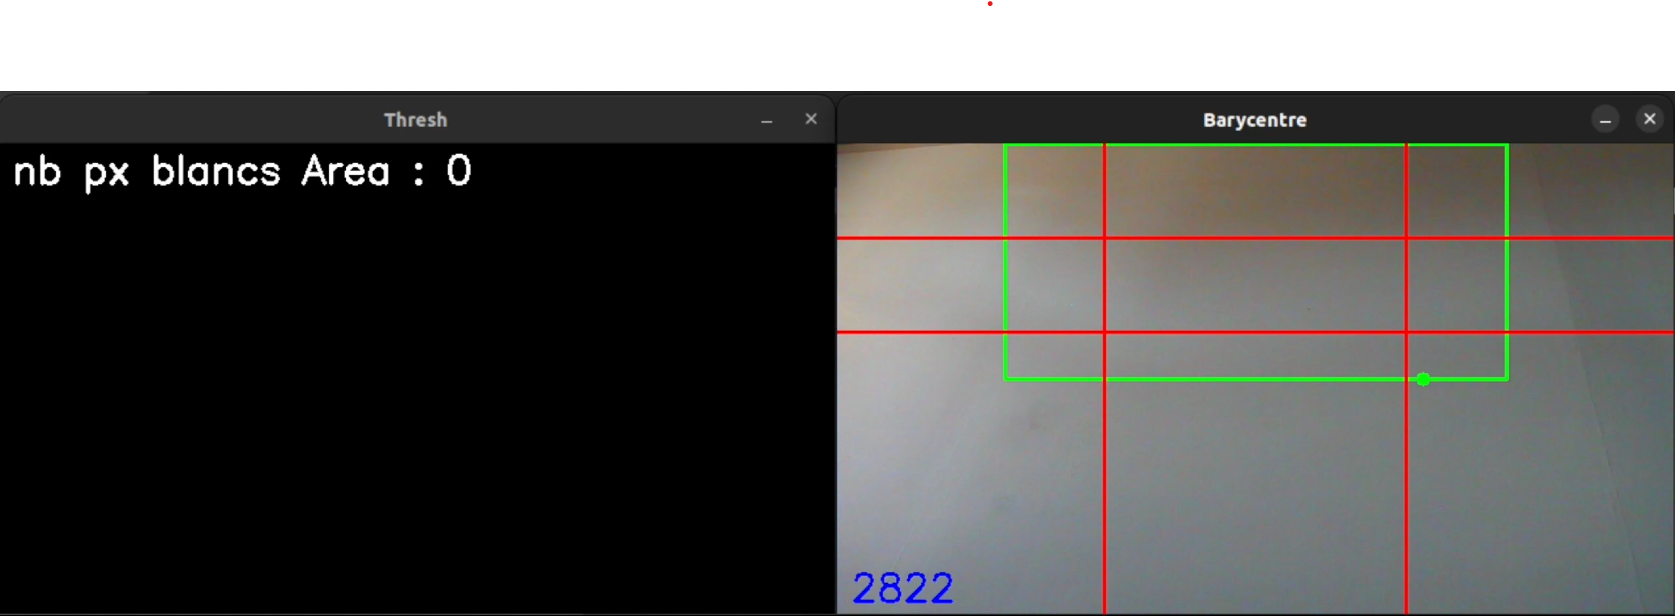
\includegraphics[width=\textwidth]{detectionDeBase.png}
      \caption{Initialisation des zones de détection}
      \label{fig:detectionDeBase}
    \end{subfigure}
    \begin{subfigure}[b]{0.48\textwidth}
      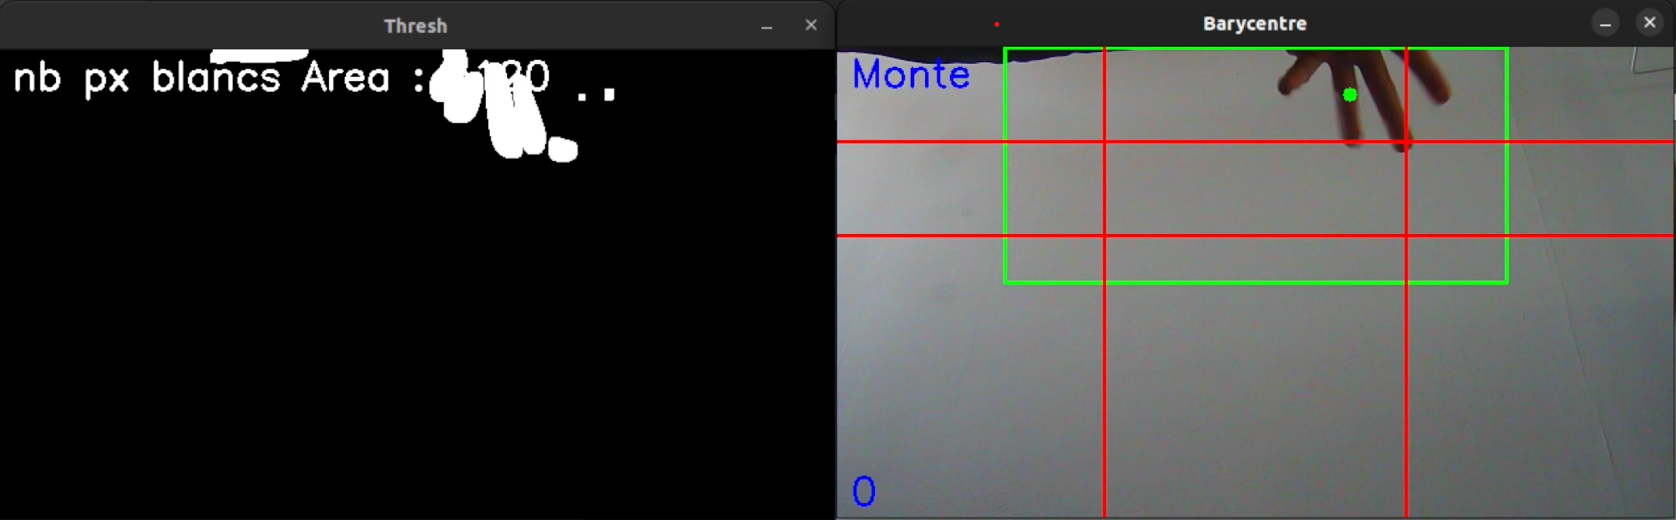
\includegraphics[width=\textwidth]{detectionHautPremier.png}
      \caption{Zone avant premier mouvement vertical}
      \label{fig:detectionHautPremier}
    \end{subfigure}

    \vspace*{7mm}

    \begin{subfigure}[b]{0.48\textwidth}
        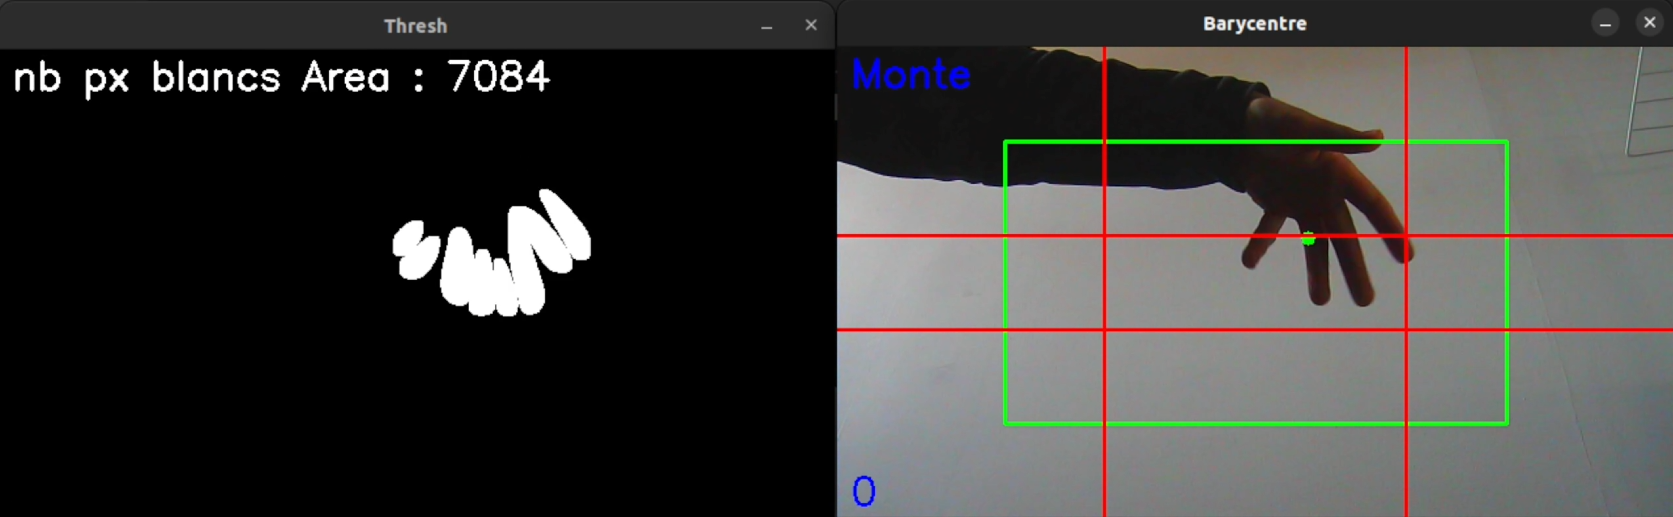
\includegraphics[width=\textwidth]{detectionHautSecond.png}
        \caption{Zones après premier mouvement vertical}
        \label{fig:detectionHautSecond}
    \end{subfigure}
    \begin{subfigure}[b]{0.48\textwidth}
        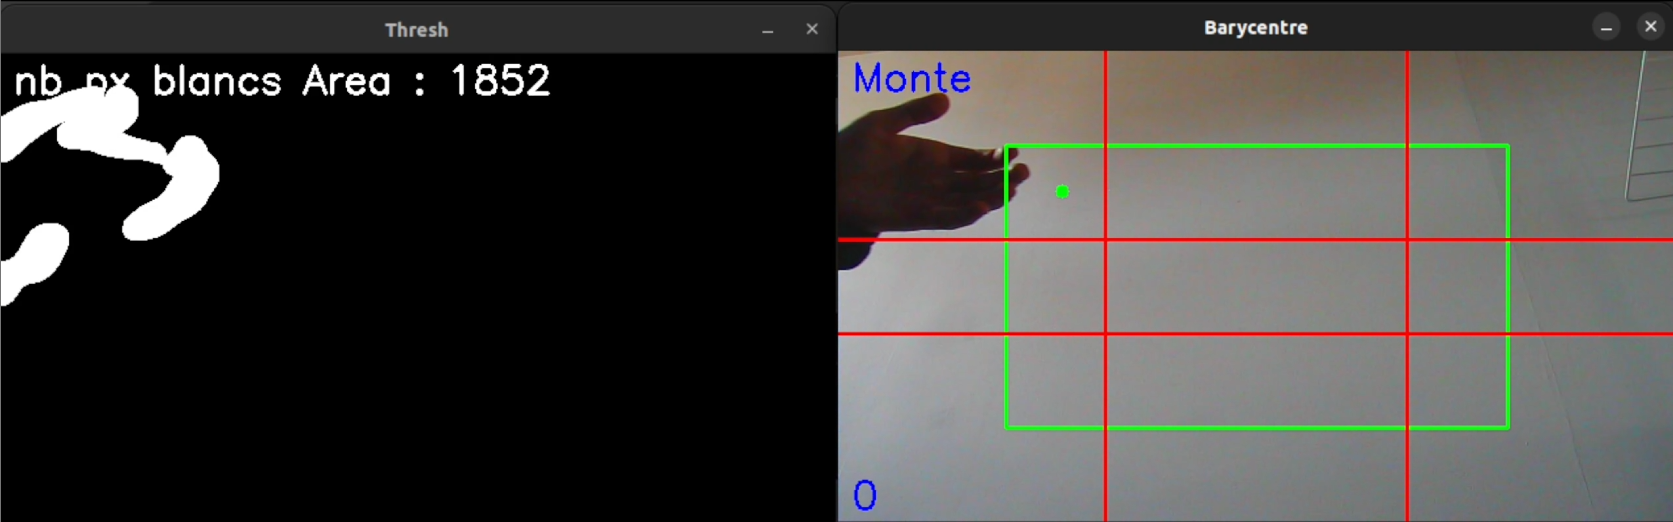
\includegraphics[width=\textwidth]{detectionHautTroisieme.png}
        \caption{Zone après second mouvement vertical}
        \label{fig:detectionHautTroisieme}
    \end{subfigure}

    \vspace*{7mm}

    \begin{subfigure}[b]{0.48\textwidth}
        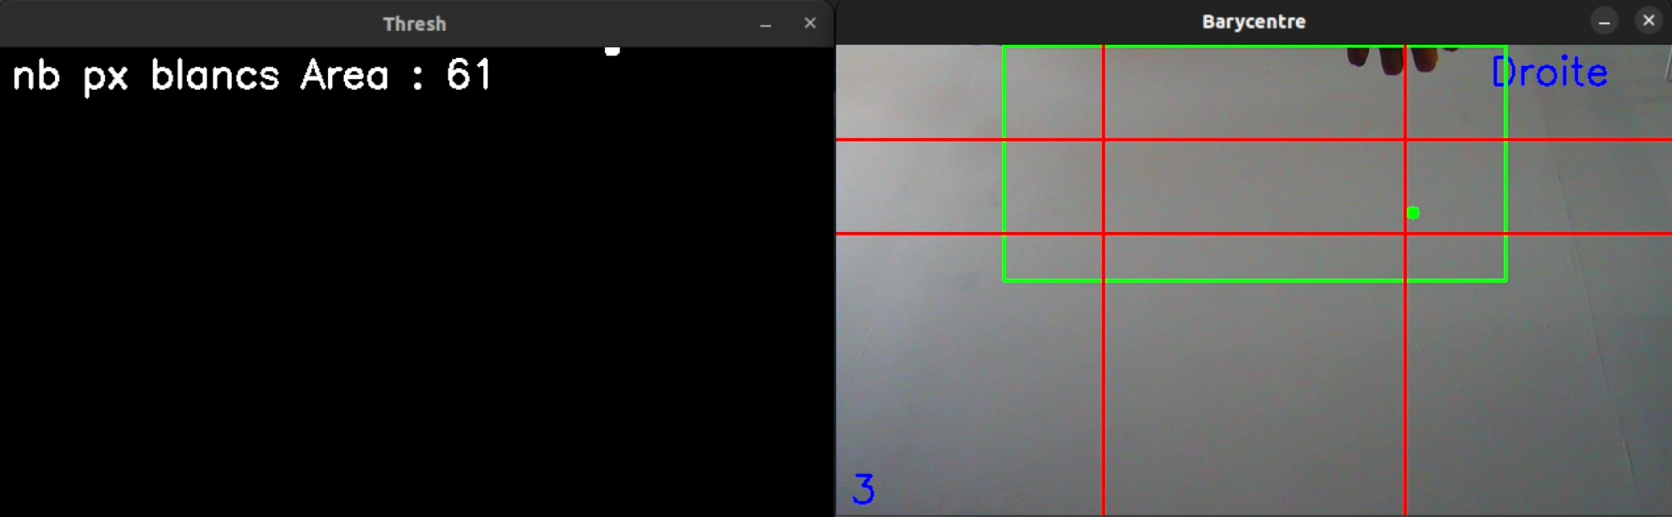
\includegraphics[width=\textwidth]{detectionDroite.png}
        \caption{Détection sur la droite}
        \label{fig:detectionDroite}
    \end{subfigure}
    \begin{subfigure}[b]{0.48\textwidth}
        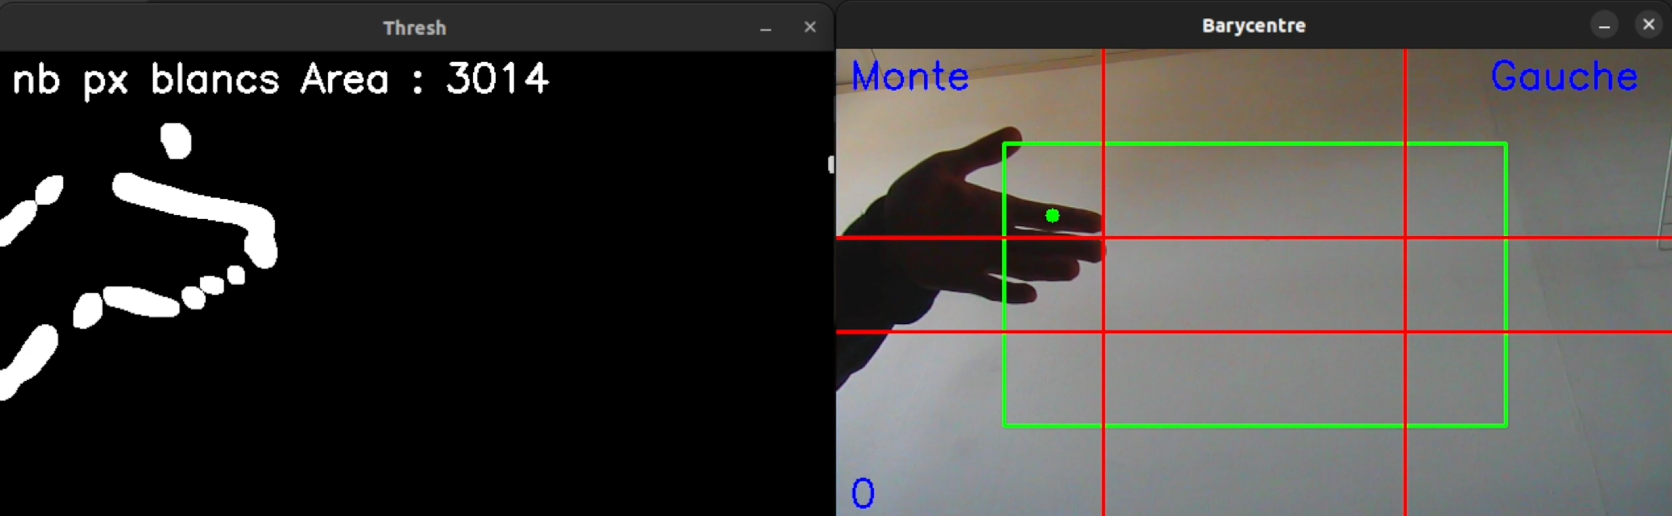
\includegraphics[width=\textwidth]{detectionGauche.png}
        \caption{Détection sur la gauche}
        \label{fig:detectionGauche}
    \end{subfigure}

    \caption{Zones de détection de mouvement}
    \label{fig:detectionArea}
  \end{figure}


%------------------------------------------------------------
\subsubsection{Capture vidéo} \label{par:capture}

Le fichier \texttt{enregistrementVideo.c} est un programme dédié à l'enregistrement des flux vidéo provenant de la mémoire partagée. Il utilise des sémaphores pour la synchronisation entre processus, la mémoire partagée pour l'accès aux images brutes, et \texttt{FFmpeg}\footnote{FFmpeg est une suite logicielle open-source puissante et polyvalente utilisée pour manipuler des fichiers multimédias (audio et vidéo). Elle permet de réaliser des tâches telles que la conversion de formats, l'encodage, le décodage, le montage, le streaming, et bien plus encore. Pour plus d'information voir \href{https://ffmpeg.org/ffmpeg.html}{la documentation en ligne}\cite{manFFmpeg} } pour encoder les vidéos dans un format compressé. Ce programme est conçu pour fonctionner de manière autonome et s'arrêter proprement en cas de signal d'interruption.


\paragraph{Initialisation du programme}
Lors de son démarrage, le programme effectue plusieurs étapes d'initialisation :
\begin{itemize}
    \item \textbf{Gestionnaire de signaux} : 
    \begin{itemize}
        \item Le programme installe un gestionnaire de signaux (\texttt{signalHandler}) pour gérer les interruptions (\texttt{SIGINT}) et les arrêts (\texttt{SIGTERM}) de manière propre.
        \item En cas de réception d'un signal, le programme termine l'enregistrement en cours et libère les ressources.
    \end{itemize}
    \item \textbf{Ouverture des sémaphores} :
    \begin{itemize}
        \item Les sémaphores nommés (\texttt{SEM\_READERS}, \texttt{SEM\_WRITER}, \texttt{SEM\_NEW\_FRAME}, etc.) sont ouverts pour synchroniser l'accès à la mémoire partagée entre les processus.
        \item Le compteur de lecteurs actifs (\texttt{SEM\_ACTIVE\_READERS}) est incrémenté pour indiquer qu'un nouveau lecteur est actif.
    \end{itemize}
    \item \textbf{Ouverture de la mémoire partagée} :
    \begin{itemize}
        \item Le segment de mémoire partagée contenant les images brutes est ouvert et mappé en mémoire virtuelle pour permettre la lecture des images.
    \end{itemize}
    \item \textbf{Préparation de la commande FFmpeg} :
    Afin d'optimiser l'utilisation de FFmpeg, on utilise sur le raspberry l'accélération matériel pour l'encodage vidéo. Pour cela, on utilise l'encoder \texttt{v4l2m2m} \cite{manFFmpegV4l2} qui permet d'utiliser le codec H.264 pour l'encodage vidéo. La commande FFmpeg est construite pour encoder les images brutes en vidéo compressée. 
    \begin{itemize}
        \item \texttt{-f rawvideo} : Spécifie que l'entrée est une vidéo brute.
        \item \texttt{fflags +discardcorrupt+genpts} : Ignore les images corrompues et génère des horodatages.
        \item \texttt{-pixel\_format bgr24} : Définit le format des pixels en BGR 24 bits.
        \item \texttt{-s 1280x720} : Définit la résolution d'entrée.
        \item \texttt{-r 25} : Définit le débit d'images d'entrée (25 FPS).
        \item \texttt{-framerate 25} : Force le débit d'image sortant (25 FPS).
        \item \texttt{-c:v h264\_v4l2m2m} : Utilise le codec H.264 pour l'encodage et l'acceleration matérielle sur le rpi. Sur une architechture x86, on peut utiliser \texttt{-c:v libx264} pour l'encodage.
        \item \texttt{-pix\_fmt yuv420p} : Définit le format des pixels en YUV 4:2:0. Ce format est optimisé pour lire les vidéos sur navigateur web.
        \item \texttt{-b:v 5M} : Définit le débit binaire de sortie à 5 Mbit/s (Meilleur débit pour de la 720p).
        \item \texttt{-an} : Désactive l'audio.
    \end{itemize}
\end{itemize}



\paragraph{Boucle principale}
Le programme entre dans une boucle principale pour capturer les images et les écrire dans le pipe standard de \texttt{FFmpeg} :
\begin{itemize}
    \item \textbf{Attente d'une nouvelle image} :
    \begin{itemize}
        \item Le programme attend qu'une nouvelle image soit disponible en utilisant le sémaphore \texttt{SEM\_NEW\_FRAME}.
    \end{itemize}
    \item \textbf{Synchronisation avec les sémaphores} :
    \begin{itemize}
        \item Le sémaphore \texttt{SEM\_WRITER} est utilisé pour bloquer l'accès en écriture pendant que l'image est lue.
        \item Le sémaphore \texttt{SEM\_READERS} est utilisé pour indiquer qu'un nouveau lecteur est en cours de lecture.
    \end{itemize}
    \item \textbf{Écriture dans le pipe FFmpeg} :
    \begin{itemize}
        \item L'image brute est lue depuis la mémoire partagée et écrite dans le pipe standard de \texttt{FFmpeg} à l'aide de la fonction \texttt{fwrite}. L'image est encodé dans une vidéo temporaire en attendant la fin de l'enregistrement.
    \end{itemize}
\end{itemize}


\paragraph{Découpage de la vidéo}
Une fois l'enregistrement terminé, la fonction \texttt{decouperVideo} est appelée pour découper la vidéo et ne conserver que la partie intéressante :
\begin{itemize}
    \item \textbf{Lecture des images de début et de fin} :
    \begin{itemize}
        \item Les images de début et de fin sont lues depuis un fichier (\texttt{PATH\_FRAMES}), qui sont écrites à la fin du processus de détection de mouvement.
        \item Si le fichier n'existe pas, des valeurs par défaut sont utilisées.
    \end{itemize}
    \item \textbf{Ajustement des images} :
    \begin{itemize}
        \item Les images sont ajustées en fonction des paramètres définis, comme le nombre de images avant le premier mouvement ou après l'absence de mouvement afin de garder une partie de la video juste avant le premier mouvement de la caméra. 
    \end{itemize}
    \item \textbf{Exécution de la commande FFmpeg} :
    \begin{itemize}
        \item Une commande \texttt{FFmpeg} est construite pour découper la vidéo en fonction des images ajustées et si besoin la réorienter dans le bon sens en fonction de l'orientation de la caméra.
        \item La vidéo temporaire (\texttt{VIDEO\_TEMP}) est utilisée comme entrée, et la vidéo finale est sauvegardée avec un nom personnalisé construit par le programme principal.
    \end{itemize}
\end{itemize}

\paragraph{Libération des ressources}
À la fin du programme, toutes les ressources utilisées sont libérées :
\begin{itemize}
    \item \textbf{Fermeture des sémaphores} : Tous les sémaphores ouverts sont fermés avec \texttt{sem\_close}.
    \item \textbf{Libération de la mémoire partagée} : Le segment de mémoire partagée est détaché (\texttt{munmap}) et fermé (\texttt{close}).
    \item \textbf{Fermeture du pipe FFmpeg} Le pipe standard vers \texttt{FFmpeg} est fermé avec \texttt{pclose}.
\end{itemize}


\paragraph{Gestion des signaux}
Le gestionnaire de signaux (\texttt{signalHandler}) permet de gérer les interruptions et les arrêts du programme :
\begin{itemize}
    \item \textbf{SIGTERM} : Arrête proprement le programme en mettant fin à la boucle principale.
    \item \textbf{SIGINT} : Interrompt immédiatement le programme.
\end{itemize}

%-----------------------------------------------------------
\subsubsection{Script démarrage automatique du programme}

Afin de démarrer le programme main au démarrage du raspberry pi, pour cela on utilise le service \texttt{rc.local} \cite{rcLocal}. Ce service permet d'exécuter après avoir initialiser tous les services du raspberry pi, le script \texttt{startSuiviGrimpeur.sh} qui va vérifier que les caméras sont bien accessible et lancer le programme. 
%-----------------------------------------------------------

\subsection{Application web}
Le serveur web est composée de deux pages web voir figure~\ref{fig:pagesWeb}, la première permet de visualiser le flux vidéo de la caméra, de la piloter et de piloter l'application. La seconde permet de visualiser les vidéos enregistrées et de les télécharger, le code de ces pages est écrit en \texttt{HTML}, \texttt{CSS} et \texttt{JAVASCRIPT} peut-être consulté sur la page \href{https://github.com/Romaiiin91/suiviGrimpeur_PDI/tree/main/server/html}{GitHub}.

\begin{figure}
  \centering
  \begin{subfigure}[b]{0.45\textwidth}
    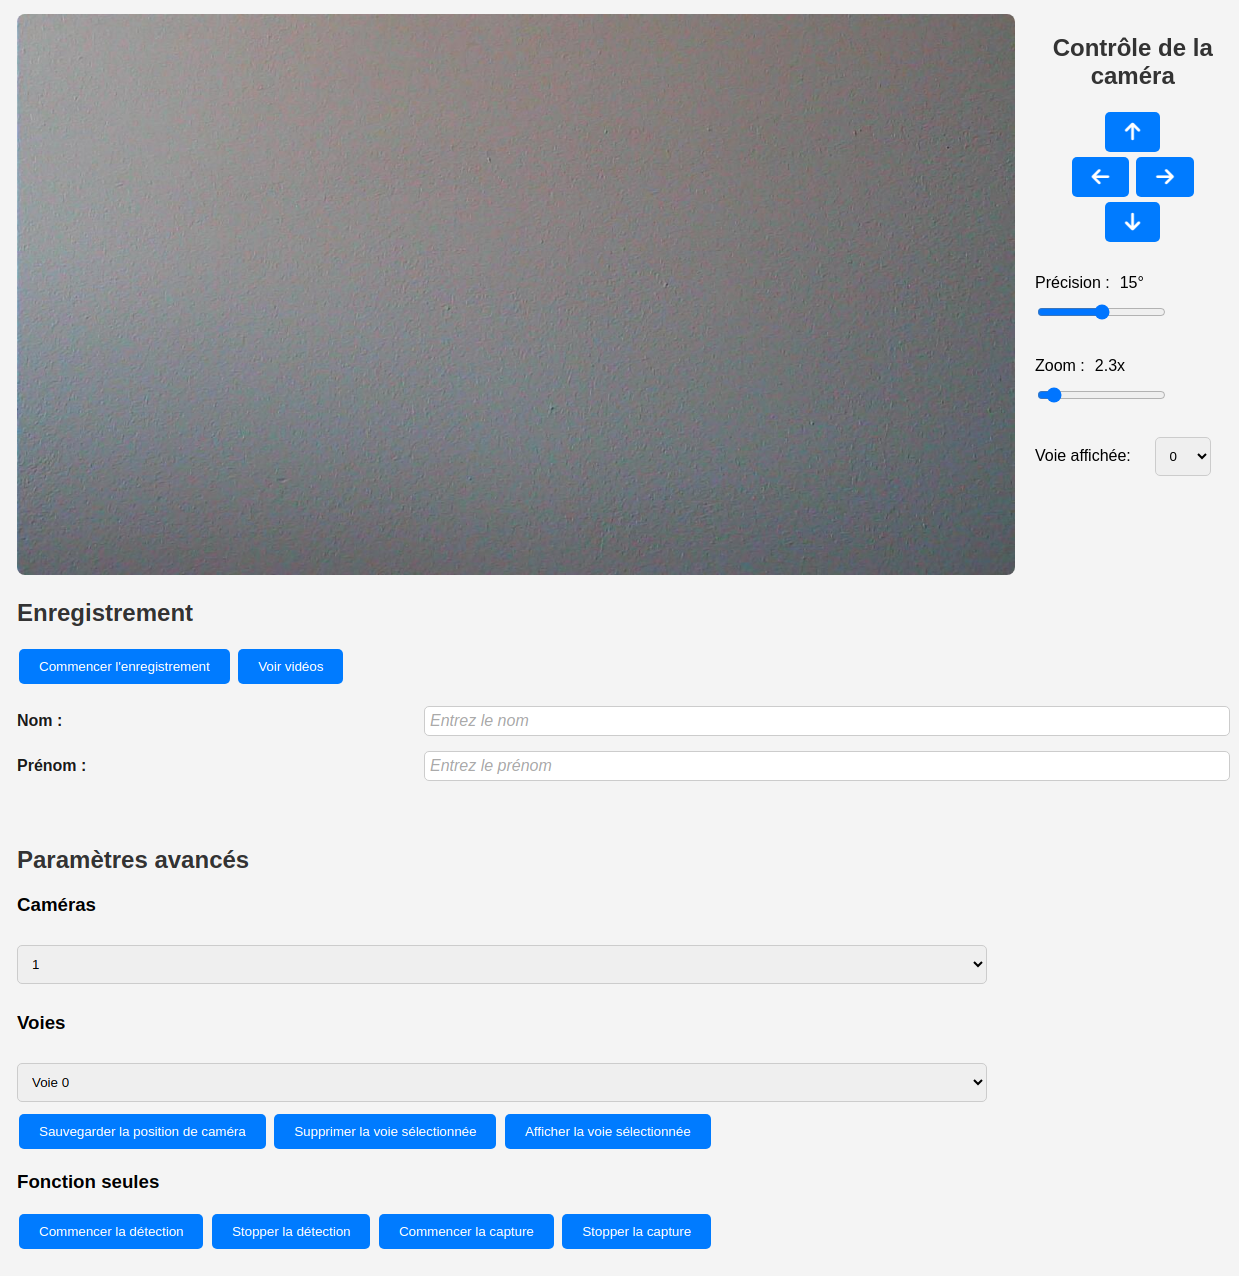
\includegraphics[width=\textwidth]{pageIndex.png}
    \caption{Index de l'application}
    \label{fig:pageIndex}
  \end{subfigure}
  \begin{subfigure}[b]{0.45\textwidth}
    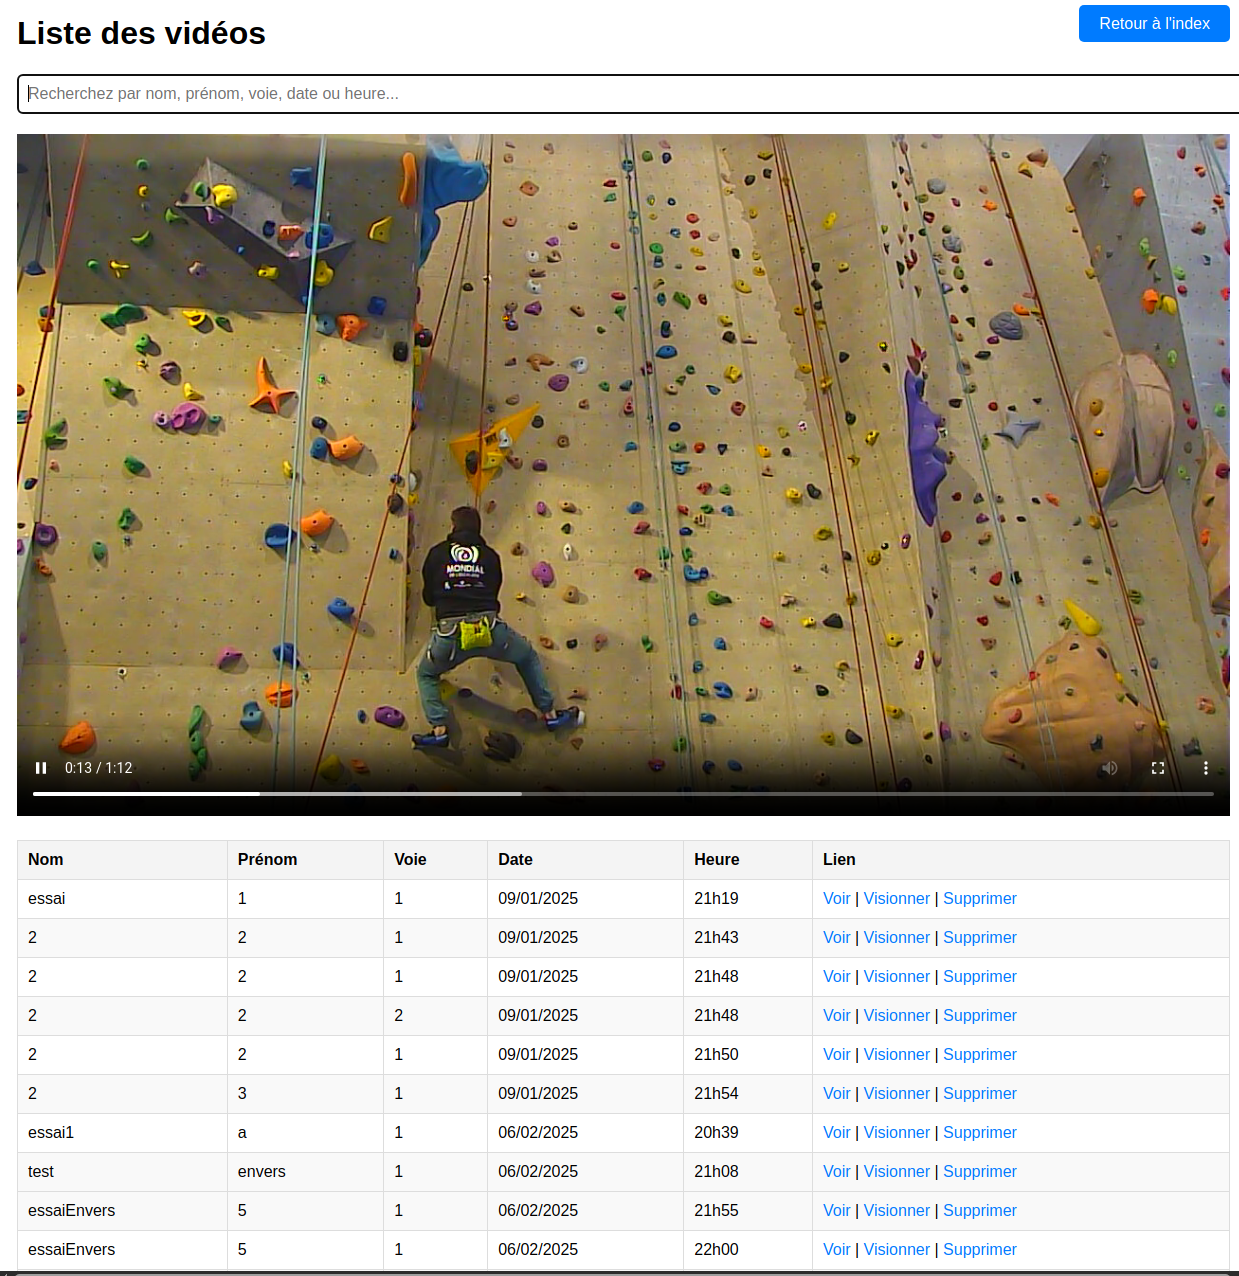
\includegraphics[width=\textwidth]{pageVideo.png}
    \caption{Page web de visualisation des vidéos}
    \label{fig:pageVideo}
  \end{subfigure}
  \caption{Pages web de l'application}
  \label{fig:pagesWeb}
\end{figure}

\subsubsection{Page web index (figure~\ref{fig:pageIndex})}
Au chargement de cette page, une fonction \texttt{javascript} permet de charger les voies disponibles dans la base de données et de les ajouter dans une liste déroulante pour permettre à l'utilisateur de sélectionner la voie qu'il souhaite visualiser. Une seconde fonction \texttt{js} charge les caméras disponibles et les ajoute dans une seconde liste déroulante. Puis le script \texttt{video.cgi} est exécuté pour afficher le flux vidéo de la caméra sélectionnée, voir la sous section \ref{sec:video.cgi} pour plus d'information.


Sur la gauche de cette page, on retrouve tout les boutons de contrôle de la caméra (haut, bas, gauche et droite) associés à un curseur pour la précision de l'angle afin de premettre un déplacement plus précis. On retrouve un second curseur pour gérer le zoom de la caméra entre 1x et 18x. La pression des boutons créent une requête \texttt{AJAX} pour exécuter le programme \texttt{action.cgi}, voir la sous section \ref{sec:action.cgi} pour plus d'information.


En dessous de ces curseurs, il y a une liste déroulante pour choisir la voie que l'on souhaite observer. À la selection d'une voie on vient changer de caméra si besoin et la positionner au bon endroit.

En dessous de la video, on retrouve un bouton pour enregistrer une vidéo avec deux champ pour entre le nom et prenom du grimpeur, un exemple de requête \texttt{AJAX} est présenté ci-contre : \texttt{http://localhost/cgi-bin/action.cgi?enrg=on\&nom=Chevalier\&prenom=Romain\&voie=0}. On récupère le nom et la voie afin de produire un nom de fichier unique et pouvoir le récupérer facilement dans la page de visualisation des vidéos.



\paragraph{Paramètres avancés}  En bas de page, on trouve les options pour configurer une nouvelle voie. Il y a une liste déroulante pour choisir la caméra, puis une seconde liste déroulante pour choisir une voie que l'on souhaite supprimer ou afficher sur l'appuie du bouton adéquat. Il y a également un bouton pour sauvegarder une nouvelle position de la caméra dans la base de données en affichant une fenêtre popup pour demander le numéro de voie. 
En addition, on peut également lancer ou stop un enregistrement seul sans suivi du grimpeur et à l'inverse, on peut lancer seulement et stopper la détection du grimpeur sans enregistrement.

\subsubsection{Programme CGI : \texttt{video.cpp}} \label{sec:video.cgi}


Le fichier \texttt{video.cpp} compilé en tant que programme CGI permet de  diffuser le flux vidéo en continu au format MJPEG (Motion JPEG) via HTTP. Il lit les images depuis le segment de mémoire partagée, les encode au format JPEG, et les envoie au client sous forme de flux MJPEG. Le programme utilise des sémaphores pour la synchronisation entre processus et gère les signaux pour une terminaison propre.


\paragraph{Initialisation du programme}
Lors de son démarrage, le programme effectue plusieurs étapes d'initialisation :
\begin{itemize}
    \item \textbf{Chargement des paramètres de la caméra} Les dimensions (\texttt{width}, \texttt{height}) et l'orientation (\texttt{orientation}) de l'image sont récupérées depuis un fichier JSON (\texttt{PATH\_CAMERA\_ACTIVE}). Ce fichier est mis à jour par le programme principal à chaque changement de caméra.
    \item \textbf{Installation des gestionnaires de signaux} :
    \item \textbf{Ouverture des sémaphores et de la mémoire partagée} :
    \item \textbf{Préparation du flux HTTP} : Le programme envoie un en-tête HTTP indiquant que le contenu est un flux MJPEG (\texttt{Content-Type: multipart/x-mixed-replace}). Cela permet de diffuser les images en continu sans interruption.
\end{itemize}

\paragraph{Boucle principale}
Le programme entre dans une boucle principale pour diffuser les images en continu :
\begin{itemize}
    \item \textbf{Attente d'une nouvelle image} : Le programme attend qu'une nouvelle image soit disponible en utilisant le sémaphore \texttt{SEM\_NEW\_FRAME}. 
    \item \textbf{Lecture de l'image depuis la mémoire partagée} : L'image brute est lue depuis la mémoire partagée et stockée dans une matrice OpenCV (\texttt{cv::Mat}).
    \item \textbf{Pré-traitement de l'image} :
    \begin{itemize}
        \item Si nécessaire, l'image est tournée en fonction de l'orientation de la caméra (\texttt{cv::rotate}).
        \item L'image est convertie du format  \textit{BGR (blue green red)} au format textit{RGB (red green blue)} à l'aide (\texttt{cv::cvtColor}) car le JPEG nécessite un profil colorimétrique en RGB.
    \end{itemize}
    \item \textbf{Encodage en JPEG} :  L'image est encodée au format JPEG à l'aide de la fonction \texttt{encode\_jpeg}, avec la librairie \texttt{libjpeg}. La qualité de l'encodage est fixée à 75 pour un bon compromis entre qualité et taille.
    \item \textbf{Envoi de l'image au client} :  L'image encodée est envoyée au client avec un en-tête indiquant la taille et le type de contenu (\texttt{Content-Type: image/jpeg}).Il envoie les images au navigateur en écrivant les en-têtes appropriés et les images encodées sur la sortie standard. 
\end{itemize}


\paragraph{Libération des ressources}
À la fin du programme, toutes les ressources utilisées sont libérées :
\begin{itemize}
    \item \textbf{Mémoire partagée} : Le segment de mémoire partagée est détaché (\texttt{munmap}) et fermé (\texttt{close}).
    \item \textbf{Sémaphores} : Tous les sémaphores ouverts sont fermés avec \texttt{sem\_close}.
    \item \textbf{Tampon JPEG} : Le tampon mémoire utilisé pour stocker les images encodées est libéré.
\end{itemize}


\subsubsection{Programme CGI : \texttt{action.c}} \label{sec:action.cgi}

Le fichier \texttt{action.c} est un programme CGI utilisé pour gérer les interactions entre le serveur web Apache et le programme principal. Il reçoit les requêtes des utilisateurs via l'interface web, les traite, et communique avec le programme principal à l'aide de la mémoire partagée et des signaux.


\paragraph{Initialisation du programme}
Lors de son démarrage, le programme effectue plusieurs étapes d'initialisation :
\begin{itemize}
    \item \textbf{Gestionnaire de fin d'exécution} : La fonction \texttt{atexit(bye)} garantit que toutes les ressources (mémoire partagée, sémaphores) sont correctement libérées à la fin du programme.
    \item \textbf{Installation des gestionnaires de signaux} :
    \begin{itemize}
        \item \texttt{SIGUSR1} : Utilisé pour recevoir une notification du programme principal indiquant que l'ordre a été traité.
        \item \texttt{SIGALRM} : Utilisé pour gérer un délai d'attente (timeout) si aucune réponse n'est reçue dans un délai de 5 secondes.
    \end{itemize}
\end{itemize}

\paragraph{Traitement des requêtes}
Le programme traite les requêtes CGI comme suit :
\begin{itemize}
    \item \textbf{Lecture de la requête} :
    \begin{itemize}
        \item Les paramètres de la requête sont récupérés depuis de la variable \texttt{QUERY\_STRING}. Cette variable d'environnement contient la chaîne de requête envoyée par le client dans l'URL après le point d'interrogation (?).
        \item Si aucun paramètre n'est reçu, le programme retourne une erreur HTTP.
    \end{itemize}
    \item \textbf{Écriture dans la mémoire partagée} :
    \begin{itemize}
        \item Le programme ouvre un segment de mémoire partagée nommé \texttt{SHM\_ORDRE}.
        \item Il écrit l'ordre reçu dans ce segment, en incluant le PID du processus CGI et les paramètres de la requête. Afin que le programme puisse répondre à ce processus en retournant un signal à la fin de l'exécution de l'ordre.
    \end{itemize}
    \item \textbf{Envoi d'un signal au programme principal} :
    \begin{itemize}
        \item Le programme principal est identifié à l'aide de son PID, lu depuis un fichier (\texttt{PATH\_FPID}).
        \item Un signal \texttt{SIGUSR1} est envoyé au programme principal pour notifier l'arrivée d'un nouvel ordre.
    \end{itemize}
    \item \textbf{Attente de la réponse} :
    \begin{itemize}
        \item Le programme attend une réponse du programme principal en utilisant la fonction \texttt{pause()} avec le signal \texttt{SIGUSR1}.
        \item Si aucune réponse n'est reçue dans un délai de 5 secondes, un signal \texttt{SIGALRM} est déclenché pour retourner un message d'erreur HTTP.
    \end{itemize}
\end{itemize}

\paragraph{Retour HTTP}
Une fois la réponse reçue, le programme retourne un message HTTP au client en fonction du statut lu dans la mémoire partagée :
\begin{itemize}
    \item \textbf{Succès (\texttt{status == 0})} : Retourne un message JSON indiquant que l'action a été exécutée avec succès.
    \item \textbf{Erreur disque (\texttt{status == -2})} : Retourne un message JSON indiquant que l'espace disque est insuffisant, code spécial pour le programme de capture vidéo.
    \item \textbf{Erreur générale} : Retourne un message JSON indiquant qu'une erreur est survenue.
\end{itemize}

\paragraph{Libération des ressources}
À la fin du programme, toutes les ressources utilisées sont libérées :
\begin{itemize}
    \item \textbf{Mémoire partagée} : Le segment de mémoire partagée est détaché (\texttt{munmap}) et fermé (\texttt{close}).
    \item \textbf{Gestion des signaux} : Les gestionnaires de signaux sont désinstallés automatiquement à la fin du programme.
\end{itemize}


\subsubsection{Page web de visualisation des vidéos (figure~\ref{fig:pageVideo})}
Cette page permet de visualiser les vidéos enregistrées, de les télécharger et de les supprimer. Elles sont répertoriées dans un tableau avec le nom du grimpeur, la voie, la date et l'heure de l'enregistrement. On peut, de plus, rechercher une video particulière à l'aide de la barre de recherche en haut de page. Avec les fonctions du navigateur, on peut lire, mettre en pause, accélérer, ralentir ou télécharger la vidéo. Enfin, on peut voir la video en haut de page en cliquant sur \texttt{voir}, la visionner dans un nouvel onglet en cliquant sur \texttt{visionner} ou la supprimer en cliquant sur \texttt{supprimer}.


%-----------------------------------------------------------

\subsection{Problèmes rencontrés}
Lors du développement des différentes étapes de l'application, plusieurs problèmes ont été rencontrés. Les deux principaux problèmes sont liés à la détection de mouvement et à l'enregistrement vidéo.

\subsubsection{Détection de mouvement}
La détection de mouvement est une étape cruciale pour le suivi du grimpeur. En première approche, j'avais décidé d'utiliser la fonction de détection de personne avec OpenCV (HOG descriptor\footnote{Voir la \href{https://docs.opencv.org/3.4/d5/d33/structcv_1_1HOGDescriptor.html}{documentation en ligne} pour plus d'information} \cite{hogDescriptor}) pour détecter le grimpeur. Mais cette méthode n'était pas très performante et perdait régulièrement la détection du grimpeur. 

Une autre approche consistait à utiliser les réseau de neurones convolutifs pour détecter le mouvement mais je me suis limité dans un premier a temps à la détection de mouvement avec OpenCV. Comme cette dernière fonctionnait bien, je n'ai pas explorer cette piste mais cette méthode aurait pu être plus performante \cite{CNNclimbertDetection}.

Avec Mr Bourdeaud'hui, nous avons fait l'hypothese que la caméra n'a pas besoin de descendre et qu'un grimpeur ira toujours vers le haut ce qui a facilité la détection des grimpeur. Nous avons donc décidé de changer de méthode et de passer à une détection de mouvement plus simple basée sur la différence d'images. Cette méthode est plus rapide et plus fiable, mais elle est sensible aux changements de luminosité, aux ombres et aux petits mouvements parasites. Pour essayer de contourner ce problème, j'ai ajouté un filtre de moyenne glissante pour lisser les mouvements et un flou gaussien afin de réduire les fausses détections. J'ai aussi ajouté une condition sur le nombre de pixel minimum avec un movement pour détecter un barycentre.

Un autre problème fut le départ du grimpeur, en effet en bas de la voie, il est difficile de distinguer le grimpeur de l'assureur. Pour résoudre ce problème, j'ai décidé de déplacer la zone de détection vers le haut de l'image pour ne regarder que le grimpeur. Et je la recentre une fois que la caméra s'est déplacée vers le haut, l'assureur n'est donc plus sur l'image.

Au départ, j'avais mis une valeur fixe pour l'angle de déplacement de la caméra, mais cela ne fonctionnait pas bien pour les différentes voies. Car en fonction du coefficient de zoom la caméra se déplaçait trop ou pas assez. J'ai donc décidé de mettre une valeur d'angle de déplacement en fonction du zoom actuel de la caméra (celui ci doit être bien défini lors de l'ajout d'une nouvelle voie). Cela a permis d'obtenir un déplacement plus précis et mieux adapté à la distance entre la voie et la caméra.

%-----------------------------------------------------------

\subsubsection{Enregistrement vidéo}

Dans un premier temps, j'avais choisi d'utiliser un encodage en H.264 avec l'encodeur \texttt{libx264} de \texttt{FFmpeg}. Cette méthode fonctionnait très bien sur une architecture matérielle puissante (ordinateur portable avec un processeur Intel Core i7 6 c\oe urs  2.6 GHz) Cependant, lorsque j'ai porté le programme sur un raspberry pi 4 (micro-processeur Cortex-A72 disposant de 4 c\oe urs à 1,5 GHz 64 bits avec 4Go de RAM), j'ai rencontré des problèmes de performances et de latence lors de l'encodage des vidéos. En effet, l'encodage en H.264 est très gourmand en ressources CPU, ce qui entraînait des ralentissements et des décalages dans le flux vidéo. Le programme d'enregistrement vidéo consommait jusqu'à \(400\ \%\) de CPU pour sortir une vidéo à 5 FPS.

Pour résoudre ce problème, après quelques recherches, j'ai découvert que le rpi possédait un encodeur matériel, j'ai décidé d'utiliser cet encodeur. Anciennement, l'encodeur vidéo était un encodeur \texttt{h264\_omx} mais sur le raspberry que je possède il a été déprécié et remplacé  par l'encodeur \texttt{v4l2m2m}\cite{v4l2}. J'ai mis beaucoup de temps à comprendre ce problème et comment utiliser l'encodeur \texttt{v4l2m2m} et comment installer FFmpeg avec cet encodeur \cite{manFFmpegV4l2}. Voir l'annexe \ref{ann:driverVideo} pour plus d'information sur le driver vidéo utilisé.

Après avoir compris comment utiliser cet encodeur, j'ai modifié le programme d'enregistrement vidéo pour utiliser l'encodeur uniquement sur le raspberry pi, c'est pour cela que j'ai laissé une option de compilation \texttt{H264} pour pouvoir compiler le programme sur un ordinateur x86 avec la librairie \texttt{libx264}.


Une fois ce problème résolu, j'ai rencontré un autre problème lié à l'encodage des vidéos qui n'était pas en mode paysage. En effet, dès lors que la vidéo était retournée, les pixels s'échangeaient de place et la vidéo était illisible. Lorsque j'ai développé cette fonctionnalité sur PC, la rotation de l'image se faisait très simplement avec la librairie \texttt{libx264} avec l'argument \texttt{-transpose} mais sur le rpi avec l'encodeur \texttt{v4l2m2m} cette option ne fonctionnait pas. J'ai du encoder la vidéo en mode paysage une première fois puis la ré-encoder avec la bonne orientation. Cette solution n'est pas optimale car chaque programme qui utilise la vidéo doit retourner l'image avant utilisation alors que le programme qui écrit l'image dans la mémoire pourrait le faire directement. Au final, j'ai profité de ce ré-encodage pour découper la vidéo en fonction des images de début et de fin pour ne garder que la partie intéressante de la vidéo.

Cependant, un problème persiste : bien que le nombre d'images par seconde en sortie soit forcé à 25 FPS, FFmpeg produit parfois un débit d'images dans un intervalle de \(25\pm 5\) fps, ce qui peut entraîner un effet de ralenti ou d'accélération de la vidéo.

\subsubsection{Problèmes liés au matériel} Lors d'un essai en salle d'escalade avec un routeur peu performant, j'ai été tributaire de la connexion wifi et le programme ne recevait que très peu d'image par seconde de la caméra. Auparavant, chaque programme (video.cgi, detection.cgi et enregistrementVideo) récupérait directement le flux vidéo via HTTP généré par la caméra. Ainsi le réseau voyait passer trois fois les mêmes informations et saturait. J'ai donc décidé de récupérer le flux vidéo une seule fois et de le partager entre les différents programmes. Cela a permis de réduire la charge réseau et d'améliorer les performances de l'application.

\subsubsection{Problèmes web} Lors de l'envoi de requêtes \texttt{AJAX} pour piloter la caméra, j'ai rencontré des problèmes de latence et de synchronisation. En effet, les requêtes étaient envoyées de manière asynchrone, ce qui entraînait des problèmes de synchronisation entre les différentes actions. Pour résoudre ce problème, j'ai ajouté des fonctions de callback pour attendre les réponses des requêtes avant d'envoyer la suivante. J'ai aussi ajouté un système de timeout pour éviter les blocages en cas de non-réponse du serveur.

Cependant, le problème n'est pas résolu. Depuis un pc, l'ordre s’exécute en 100 ms dans toutes les directions mais sur le raspberry pi, l'ordre vers le haut s'exécute aussi en moins de 100ms mais les autres ordres attend le signal \texttt{SIGALRM} fixé a 500ms car l'ordre est bien traité avant ces 500ms. 

Voir cette \href{https://youtu.be/0Z2cE6WyGWY}{vidéo} pour voir le problème en action. Dans un premier temps, on fait le test sur le raspberry et dans un second sur un pc. On voit que sur le pc, les ordres sont exécutés en moins de 100ms alors que sur le raspberry, les ordres sont exécutés en 500ms sur la droite de l'écran dans l'inspecteur réseau.


%-----------------------------------------------------------
\section{Tests et résultats}
Je suis allé plusieurs fois dans la salle d'escalade afin de tester le programme en conditions réelles. J'ai pu tester la détection de mouvement, le suivi du grimpeur, l'enregistrement vidéo et la visualisation des vidéos. J'ai aussi pu affiner les paramètres de détection. On trouve en figure~\ref{fig:testDetection} un exemple de détection du grimpeur en mode paysage et en mode portrait. Au final, lors de l'essai final à Mons le programme fonctionnait bien. J'ai pu enregistrer des vidéos de grimpeurs, les visualiser et les télécharger ainsi que paramétrer les voies. Pour voir un exemple de détection voir cette \href{https://youtu.be/jRj4fich-2w}{vidéo}.

\begin{figure}[!ht]
     \begin{center}
        \begin{subfigure}[t]{0.70\textwidth}
            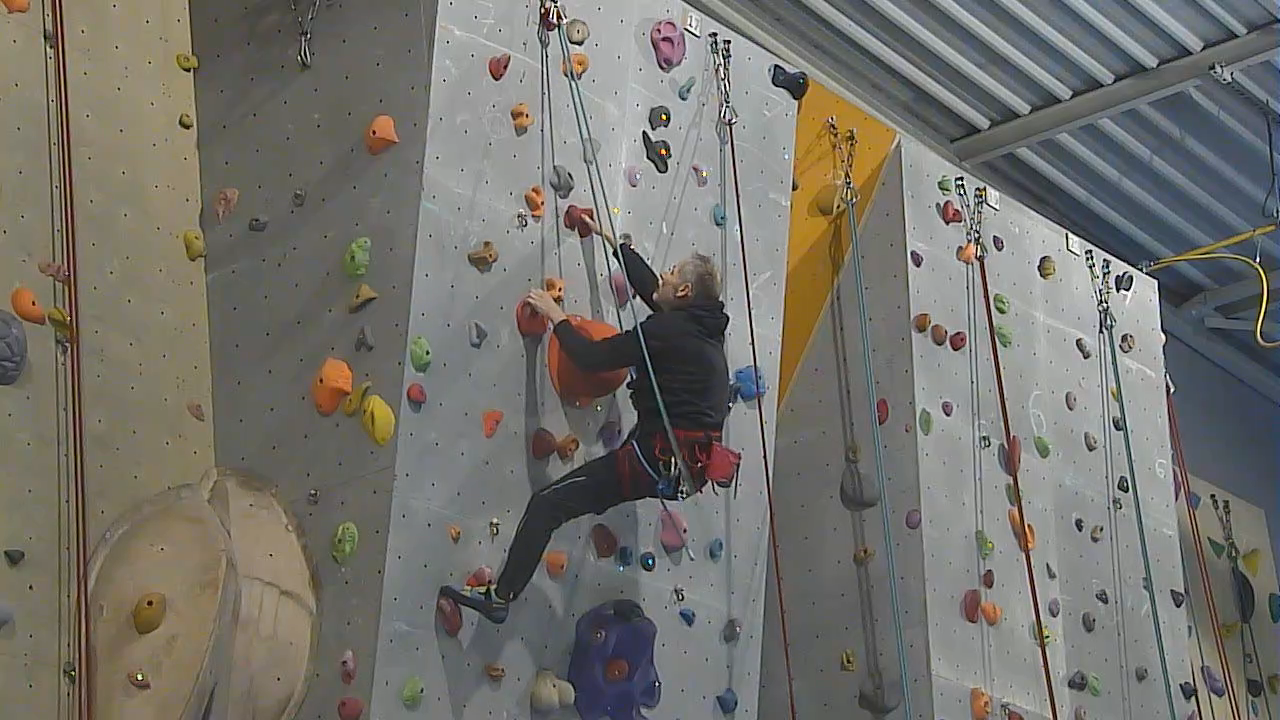
\includegraphics[width=\textwidth]{exemplePaysage.png}
            \caption{Détection du grimpeur en mode paysage}
            \label{fig:test1}
        \end{subfigure}
        \begin{subfigure}[t]{0.22\textwidth}
            \centering
            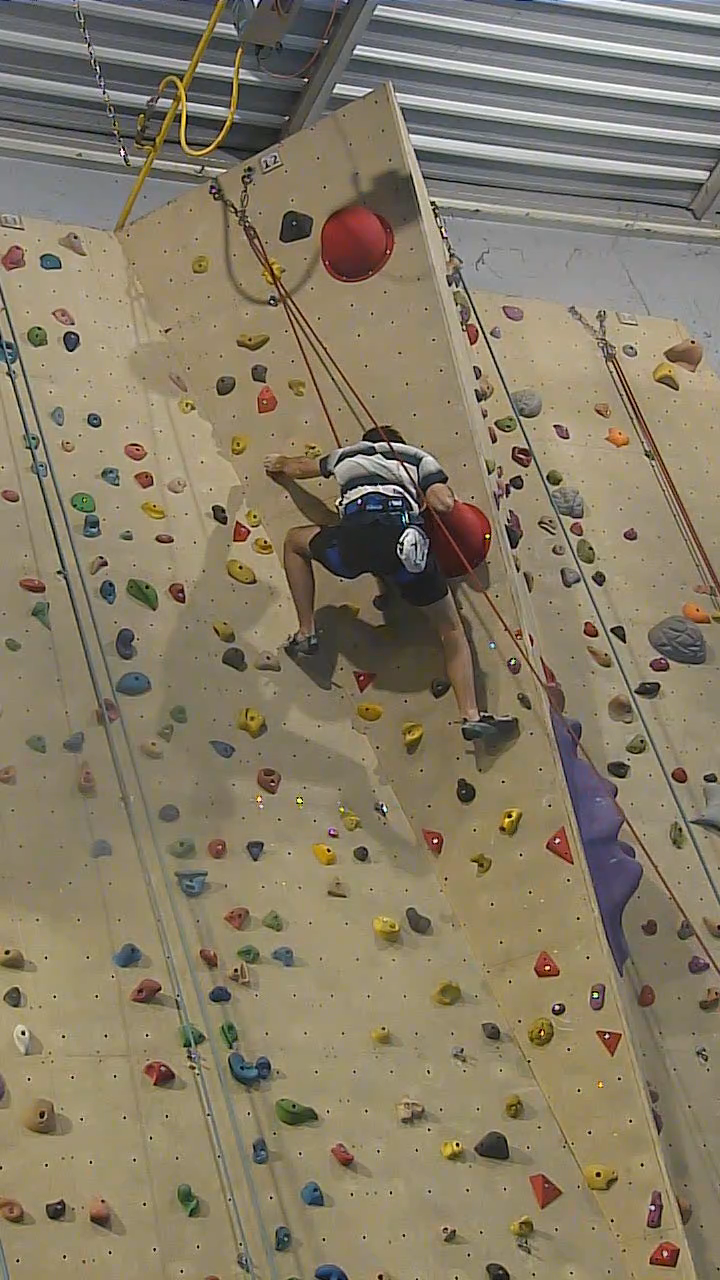
\includegraphics[width=\textwidth]{exemplePortrait.png}
            \caption{Détection du grimpeur en mode portrait}
            \label{fig:test2}
        \end{subfigure}

        \begin{subfigure}[b]{0.45\textwidth}
            \centering
            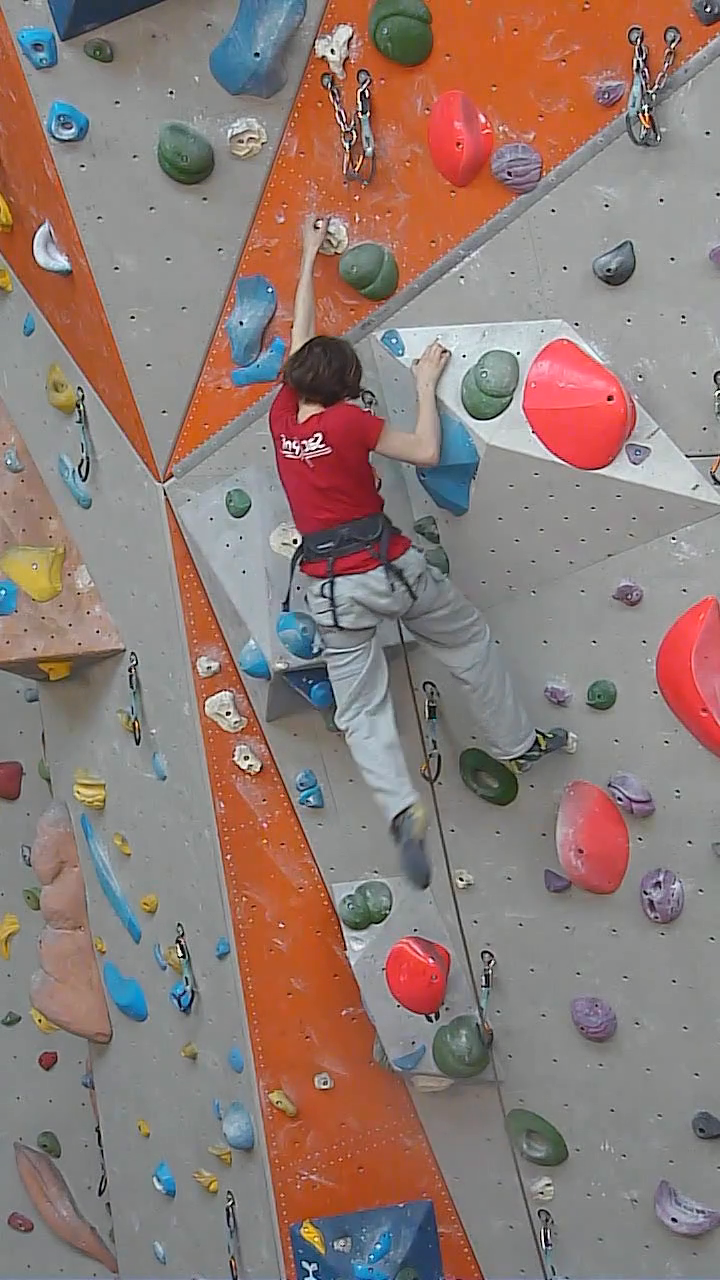
\includegraphics[width=0.6\textwidth]{VinesioGrimpe.png}
            \caption{Détection du grimpeur à Mons}
            \label{fig:test3}
        \end{subfigure}
        \begin{subfigure}[b]{0.45\textwidth}
            \centering
            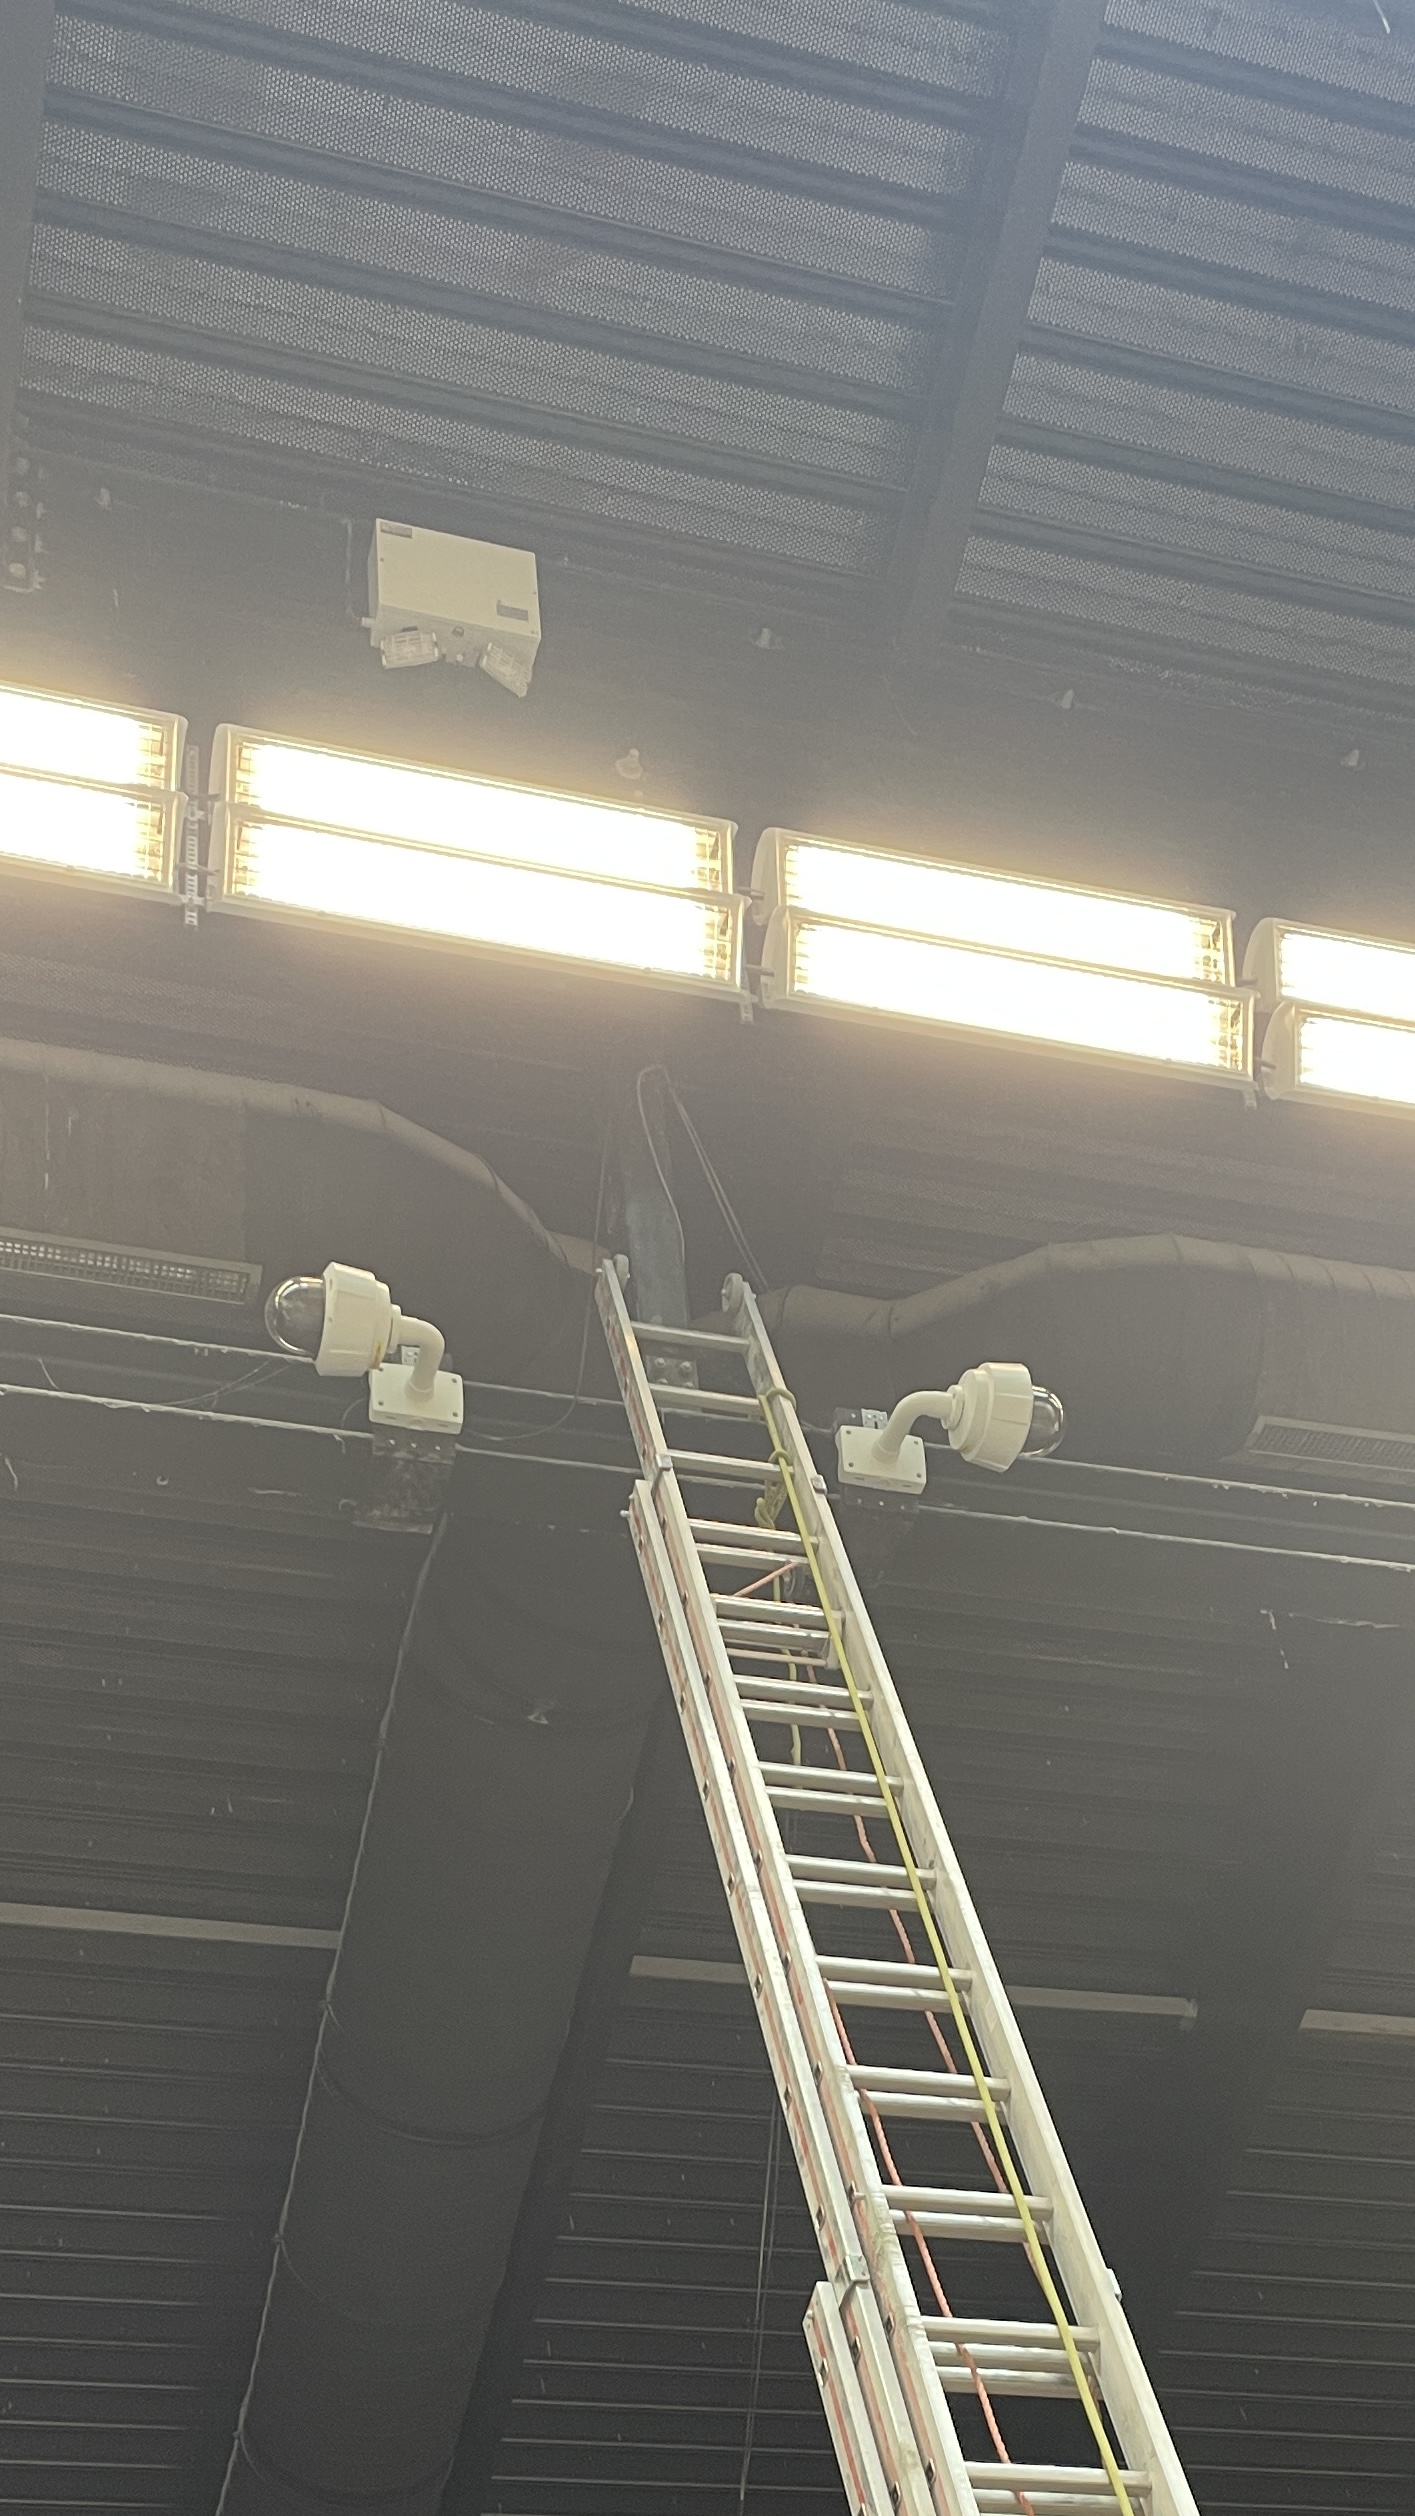
\includegraphics[width=0.6\textwidth]{instalCamera.JPEG}
            \caption{Détection du grimpeur en mode portrait}
            \label{fig:test4}
        \end{subfigure}
        \caption{Test et installation}
        \label{fig:testDetection}
     \end{center}
\end{figure}

\section{Perspectives d'amélioration}
L'application fonctionne correctement, mais il reste des améliorations à apporter pour la rendre plus robuste et plus performante. Voici quelques pistes d'amélioration pour le futur :
\begin{itemize}
  \item Amélioration de l'interface Web, avoir une interface plus intuitive et plus ergonomique.
  \item Reformater le code et tout traduire en anglais
  \item Sur l'écran du Raspberry Pi, afficher un meilleur status de l'execution de l'application.
  \item Utiliser les boutons du Raspberry Pi pour relancer l'application et l'écran tactile. 
  \item Ajouter un système de notification pour les erreurs.
  \item Mieux gérer le stockage des vidéos.
  \item Serveur accessible depuis internet pour voir les vidéos (chiffrement des données).
  \item Ajouter un système de détection de chute.
  \item Ajouter la possibilité d'enregistrer avec les deux caméras en même temps, voir si un changement de matériel est nécessaire.
  \item Changer l'implémentation des sémaphores pour synchroniser les nouvelles images. (Par exemple, utiliser 4 buffers et changer le buffer d'écriture le temps que les processus le lisent et swap les buffers). 
\end{itemize}




\section{Conclusion}
Ce projet a permis de développer une application complète et fonctionnelle pour le suivi automatisé des grimpeurs dans une salle d'escalade à l'aide de caméras motorisées. En combinant des technologies variées telles que la détection de mouvement, l'encodage vidéo, et une interface web intuitive, nous avons pu répondre aux objectifs initiaux tout en surmontant plusieurs défis techniques.

Les tests réalisés en conditions réelles ont démontré la robustesse et l'efficacité du système, bien que des améliorations soient encore possibles, notamment en termes d'ergonomie, de gestion des ressources, et d'optimisation des performances. Les perspectives d'amélioration identifiées ouvrent la voie à des évolutions futures pour rendre l'application encore plus performante et adaptée aux besoins des utilisateurs.

En conclusion, ce projet offre une solution innovante et pratique pour l'analyse et le suivi des performances des grimpeurs.

%-----------------------------------------------------------

\clearpage
\newpage
\printbibliography[nottype=none]  


% %-----------------------------------------------------------
\clearpage
\newpage


\section*{Annexes}
\addcontentsline{toc}{section}{Annexes}

\appendix

\startcontents[sections]
\printcontents[sections]{l}{1}{\setcounter{tocdepth}{2}}


\section{Github}

Le lien du dépôt GitHub contenant le code source de l'application est le suivant \href{https://github.com/Romaiiin91/suiviGrimpeur_PDI}{page GitHub}.
      
\section{Driver vidéo} \label{ann:driverVideo}
\begin{lstlisting}[caption={Propriétes du driver vidéo utilisé pour encoder le flux vidéo},captionpos=b]
    pi@raspberrypi:~ $ v4l2-ctl --device=/dev/video11 --all
    Driver Info:
        Driver name      : bcm2835-codec
        Card type        : bcm2835-codec-encode
        Bus info         : platform:bcm2835-codec
        Driver version   : 6.6.74
        Capabilities     : 0x84204000
            Video Memory-to-Memory Multiplanar
            Streaming
            Extended Pix Format
            Device Capabilities
        Device Caps      : 0x04204000
            Video Memory-to-Memory Multiplanar
            Streaming
            Extended Pix Format
    Media Driver Info:
        Driver name      : bcm2835-codec
        Model            : bcm2835-codec
        Serial           : 0000
        Bus info         : platform:bcm2835-codec
        Media version    : 6.6.74
        Hardware revision: 0x00000001 (1)
        Driver version   : 6.6.74
    Interface Info:
        ID               : 0x0300001a
        Type             : V4L Video
    Entity Info:
        ID               : 0x0000000f (15)
        Name             : bcm2835-codec-encode-source
        Function         : V4L2 I/O
        Pad 0x01000010   : 0: Source
          Link 0x02000016: to remote pad 0x1000012 of entity 'bcm2835-codec-encode-proc' (Video Encoder): Data, Enabled, Immutable
    Priority: 2
    Format Video Capture Multiplanar:
        Width/Height      : 32/32
        Pixel Format      : 'H264' (H.264)
        Field             : None
        Number of planes  : 1
        Flags             : 
        Colorspace        : Rec. 709
        Transfer Function : Default
        YCbCr/HSV Encoding: Default
        Quantization      : Default
        Plane 0           :
           Bytes per Line : 0
           Size Image     : 524288
    Format Video Output Multiplanar:
        Width/Height      : 32/32
        Pixel Format      : 'YU12' (Planar YUV 4:2:0)
        Field             : None
        Number of planes  : 1
        Flags             : 
        Colorspace        : Rec. 709
        Transfer Function : Default
        YCbCr/HSV Encoding: Default
        Quantization      : Default
        Plane 0           :
           Bytes per Line : 64
           Size Image     : 3072
    \end{lstlisting}

\section{Notice utilisation}
\begin{figure}[!ht]
    \centering
    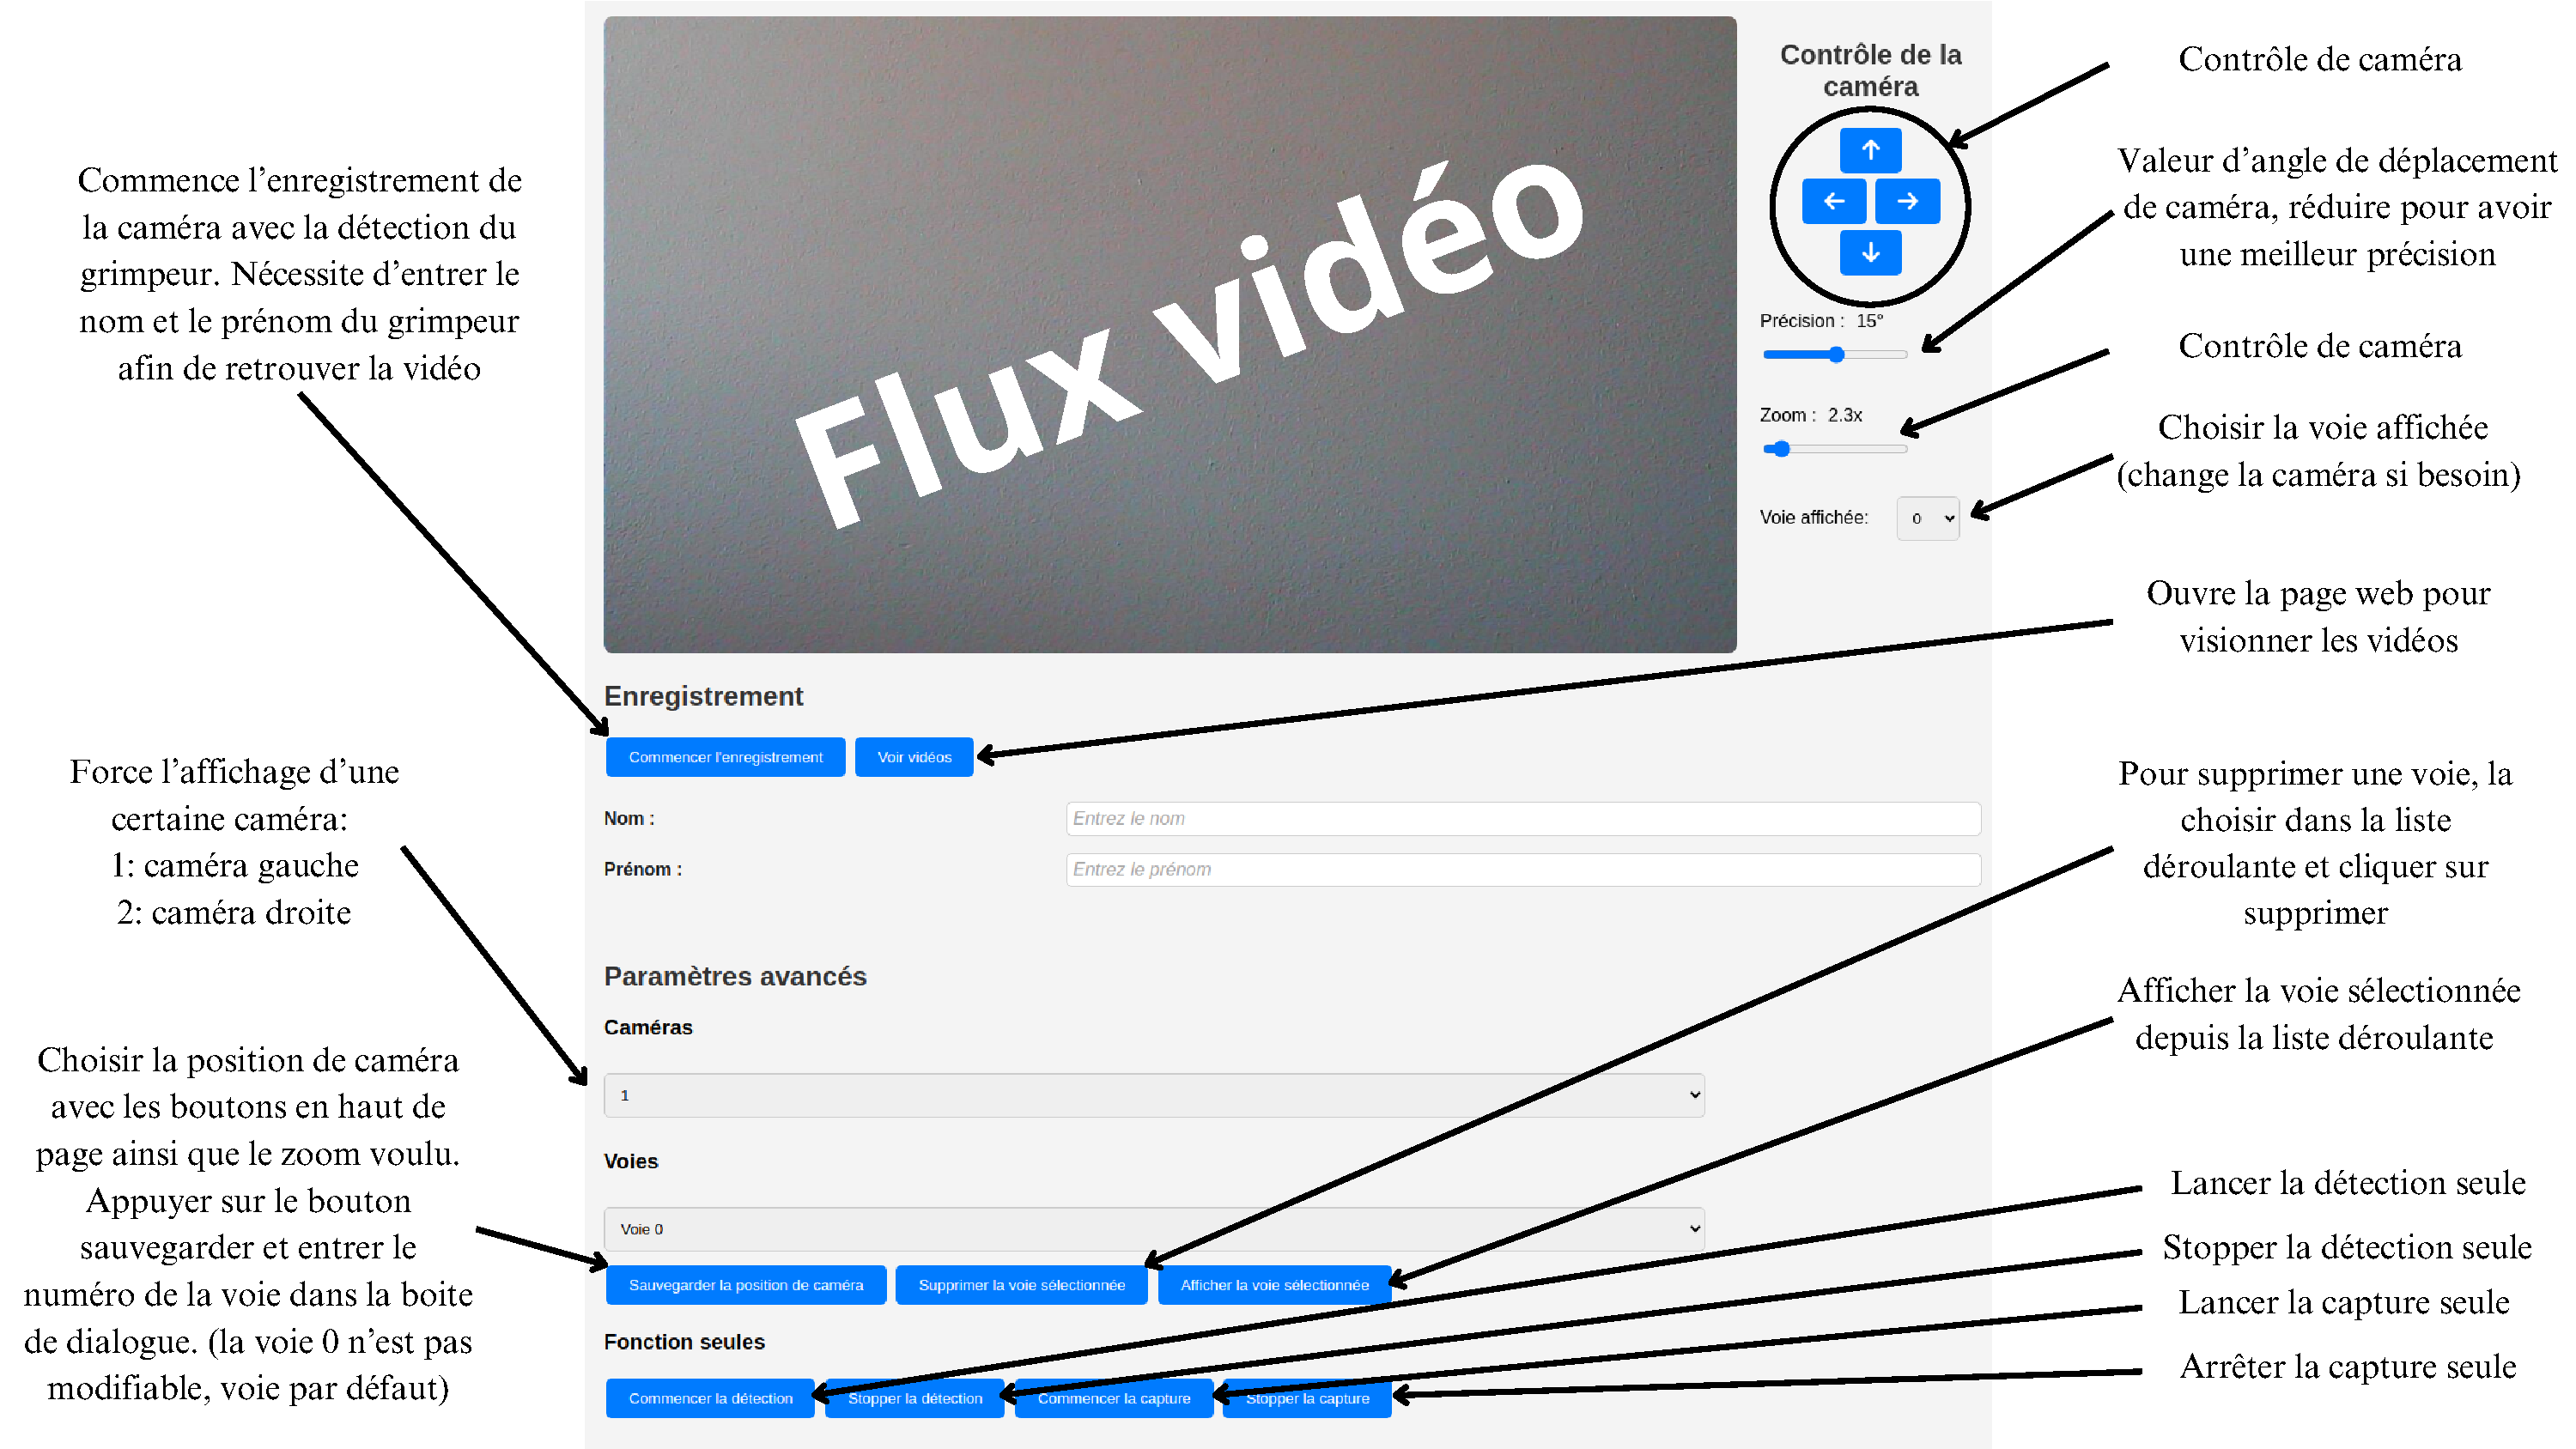
\includegraphics[width=\textwidth]{noticeSuiviGrimpeur.pdf}
    \caption{Notice d'utilisation}
    \label{fig:noticeUtilisation}
\end{figure}

\end{document}
